\documentclass{article}
\usepackage {mathtext}
\usepackage{amsmath}
\usepackage [russian] {babel}
\usepackage{caption}
\captionsetup[table]{position=t,justification=raggedleft,slc=off}
\setlength{\abovecaptionskip}{0pt}
\usepackage {geometry}
\usepackage {amssymb}
\usepackage{graphicx}
\usepackage{subfigure}
\geometry{margin=1in}
\graphicspath{{pic/}}
\title{Лабораторная работа №3.6.1. \\ \textbf{Спектральный анализ электрических сигналов}}
\author{Павел Рудачихин, Б04-507}
\date{08.09.2026}
\begin {document}
\maketitle{}


\section {Аннотация} 
	\hspace{4mm} Целью данной работы являются получение спектров сигналов различной формы, проверка соотношений неопределённостей, получение и спектральный анализ модулированных по амплитуде и фазе сигналов, определение коэффициентов передачи RC-цепочки, измерение её постоянной времени. Для этого в работе используются генератор сигналов произвольной формы АКИП-3409/4, цифровой USB-осциллограф АКИП-72205А, подключённый к ПК с ПО <<Picoscope-6>>, RC-цепочка. 

\section {Теоретическое введение}
	
	\subsection {Преобразование Фурье}
	
		\hspace{4mm} Согласно теореме Фурье, любая периодическая функция может быть представлена в виде суммы или ряда гармонических функций с кратными частотами:
		
		\begin{equation}
			f(t) = \frac{A_0}{2} + \sum_{n=1}^{\infty} A_n \cos(2\pi \nu_n t) + B_n \sin(2\pi \nu_n t)
		\end{equation}
		
		\begin{equation}
			f(t) = \frac{a_0}{2} + \sum_{n=1}^{\infty} a_n \cos(2\pi \nu_n t + \phi_n)
		\end{equation}
		
		где 
		
		\begin{equation}
			A_n = \frac{2}{T} \int_0^Tf(t)\cdot \cos(2\pi \nu_n t) dt, \  \ B_n = \frac{2}{T} \int_0^Tf(t)\cdot \sin(2\pi \nu_n t) dt, \  \ a_n = \sqrt{A_n^2 + B_n^2}, \ \ \tg\phi_n = \dfrac{B_n}{A_n}
		\end{equation}
		
		С помощью формулы Эйлера $e^{ix} = \cos x + i \sin x$ можно записать лаконично:
		
		\begin{equation}
			f(t) = \sum_{-\infty}^{+\infty} c_n \exp(in\omega t)
		\end{equation}
		
		где $\omega = 2\pi/T, \ c_n = T^{-1}\int_0^Tf(t) \exp(in\omega t)dt $
		
		Спектр функции $f(t)$ -- совокупность всех частот $\nu_n$ и соответствующих им амплитуд $a_n$ и фаз $\phi_n$. В данной работе исследуется спектр электрического сигнала, т.е. спектр изменяющегося во времени напряжения $U(t)$.
		
		В случае непериодической функции спектр становится непрерывным, а разложение происходит в интеграл Фурье. 
		

		
		
		
		Преобразование Фурье -- операция, при которой функции $f(t)$ ставится в соответствие её ряд (интеграл) Фурье. Это преобразование биективно. Однако, как правило, при спектральном анализе электрических сигналов измеряется амплитуда, а информация о фазах теряется, поэтому разные сигналы могут иметь одинаковые амплитудные спектры.
	
	\subsection {Соотношение неопределённостей}
	
		\hspace{4mm} Если у сигнала $f(t)$ есть характерное время $\Delta t$ (период, длительность импульса, время нарастания и т.п.), то в спектре $a(\nu)$ будет наблюдаться характерный масштаб $\Delta \nu$ (расстояние между пиками, ширина спектра, ширина пика и т.п.), причём
		
		\begin{equation}
			\Delta \nu \cdot \Delta t \sim 1
		\end{equation}
	
	\subsection{Цифровой спектральный анализ}
	
		\hspace{4mm} В данной работе спектральный анализ производится с помощью USB-осциллографа и персонального компьютера, т.е. цифровым методом.
		
		Сначала сигнал оцифровывается: значения напряжения считываются с определённой частотой -- частотой дискретизации $\nu_{дискр}$. Для надёжного получения спектра важно, чтобы частоты были меньше частоты дискретизации (по теореме Котельникова хотя бы в два раза). Дискретный сигнал раскладывается в спектр с помощью быстрого преобразования Фурье.
		
		Для анализа считывается лишь отрезок сигнала -- окно, из-за чего возникают искажения спектра -- краевые эффекты. Для их подавления регистрируемая функция умножается на оконную функцию (см. рис. 1), которая придаёт значениям исходной функции разный вес в пределах окна. Так, в данной работе использовано окно с плоской вершиной, которое лучше всего подходит для измерения амплитуд.
		
		\begin{figure}[h!]
			\centering
			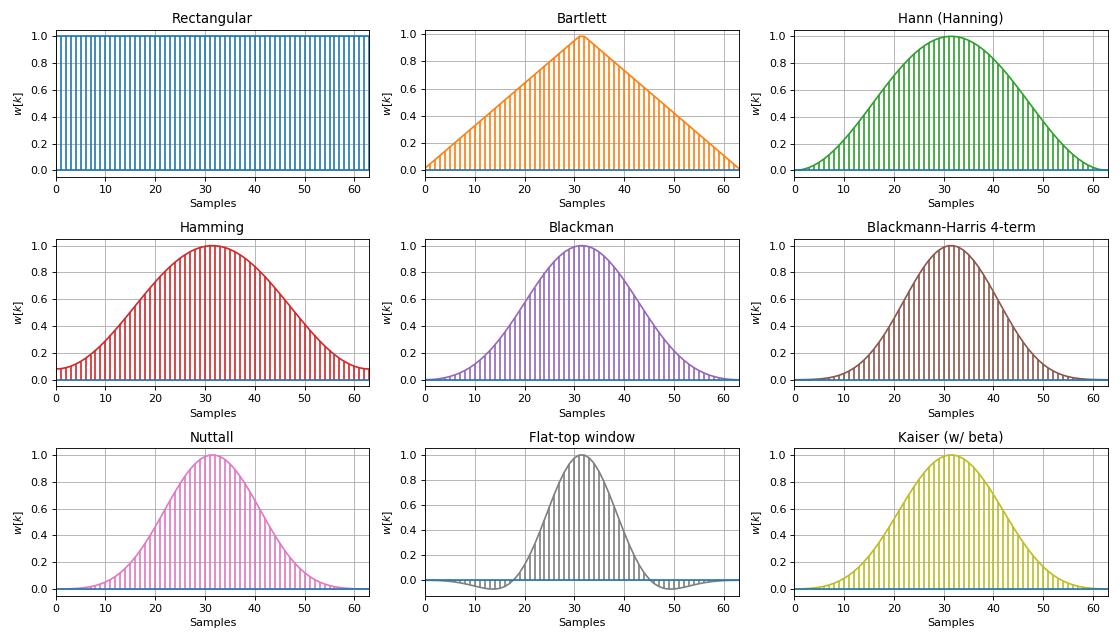
\includegraphics[width=\linewidth]{windows}
			\caption{Оконные функции}
			\label{fig:window}
		\end{figure}
		 
		 Таким образом, в данной работе будет использовано быстрое преобразование Фурье с flat-top окном.
		
		
	\subsection{Спектр прямоугольных импульсов}
	
	Выразим амплитуды гармоник периодических прямоугольных импульсов с периодом $T$ и длительностью $\tau$:
	
	\begin{equation}
		c_n =  \frac{1}{T}\int_{-\tau/2}^{\tau/2}a_0 \exp(in\omega t)dt = \dfrac{\sin(\pi n \tau/T)}{\pi n}
	\end{equation}
	
	\subsection{Амплитудная модуляция}
	
	Рассмотрим амплитудно-модулированный гармонической функцией сигнал
	
	\begin{equation}
		f(t) = a(t)\cos\omega t, \ a(t) = a_0(1 + m\cos\Omega t)
	\end{equation}
	
	где $m$ - глубина модуляции.
	
	По формуле произведения косинусов
	
	\begin{equation}
		f(t) = a_0\cos(\omega t) + \frac{ma_0}{2}\cos(\omega + \Omega)t  + \frac{ma_0}{2}\cos(\omega - \Omega)t
	\end{equation}
	
	откуда следует, что у АМ-сигнала есть три гармоники - основная и две боковых.
	
	
	\subsection{Фазовая модуляция}
	
	Рассмотрим фазово-модулированный гармонической функцией сигнал
	
	\begin{equation}
		f(t) = a_0\cos(\omega t + \phi(t)), \ \phi(t) =  m\cos\Omega t
	\end{equation}
	
	где $m$ - глубина модуляции.
	
	По формуле косинуса суммы при $m \ll 1$ имеем
	
	\begin{equation}
		f(t) = a_0\cos(\omega t) + \frac{ma_0}{2}\cos((\omega + \Omega)t + \frac{\pi}{2})  + \frac{ma_0}{2}\cos((\omega - \Omega)t+ \frac{\pi}{2})
	\end{equation}
	
	откуда следует, что действительный спектр ФМ-сигнала с малой глубиной модуляции не отличим от спектра АМ-сигнала.
	
	
	\subsection{RC-цепочка}
	
	Ёмкостное сопротивление конденсатора зависит от его ёмкости и частоты переменного тока $X = 1/\omega C$. Рассматривая RC-цепь как делитель напряжения, имеем
	
	\begin{equation}
		\frac{U_{out}}{U_{in}} = \frac{Z_C}{Z} = \frac{X_C}{\sqrt{R^2 + X_C^2}} =\frac{1}{\sqrt{1 + (\omega RC)^2}} 
	\end{equation}
	
	
\section{Описание установки}
	
	\begin{figure}[h!]
		\centering
		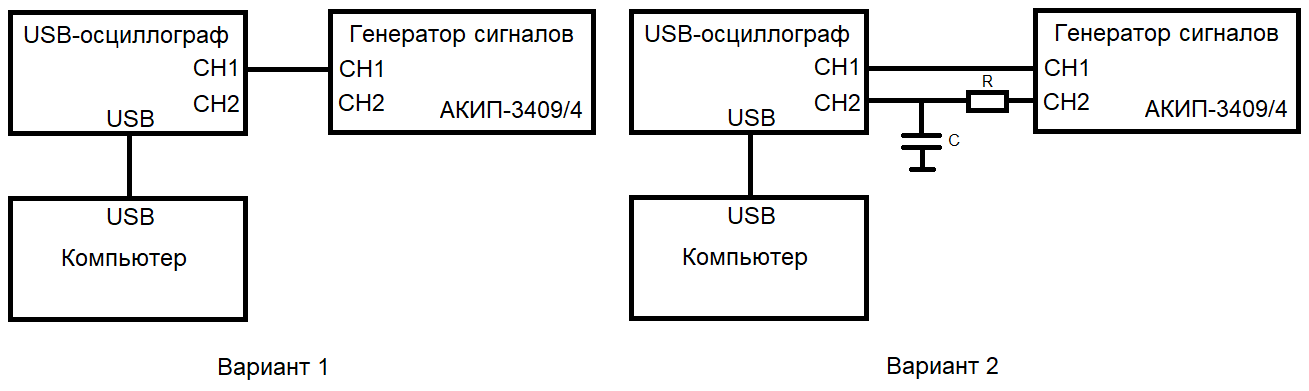
\includegraphics[width=\linewidth]{scheme}
		\caption{Схема установки}
		\label{fig:scheme}
	\end{figure}
	
	
	Схема установки довольно проста. Первый вариант в пояснении не нуждается. Второй вариант содержит RC-цепочку: R = 3 кОм, С = 1 нФ. Постоянная времени $\tau_{RC} = 3 \ мкс$.
	
\section{Результаты и обсуждения}

	\subsection{Периодические прямоугольные импульсы}
	
		\hspace{4mm} На генераторе была установлена генерация прямоугольных импульсов частотой $\nu_r = 1\ кГц$ и с длительностью импульса $\tau = 50 \ мкс$, коэффициент заполнения 5\% (см. рис. \ref{fig:1}).
		
		\begin{figure}[h!]
			\centering
			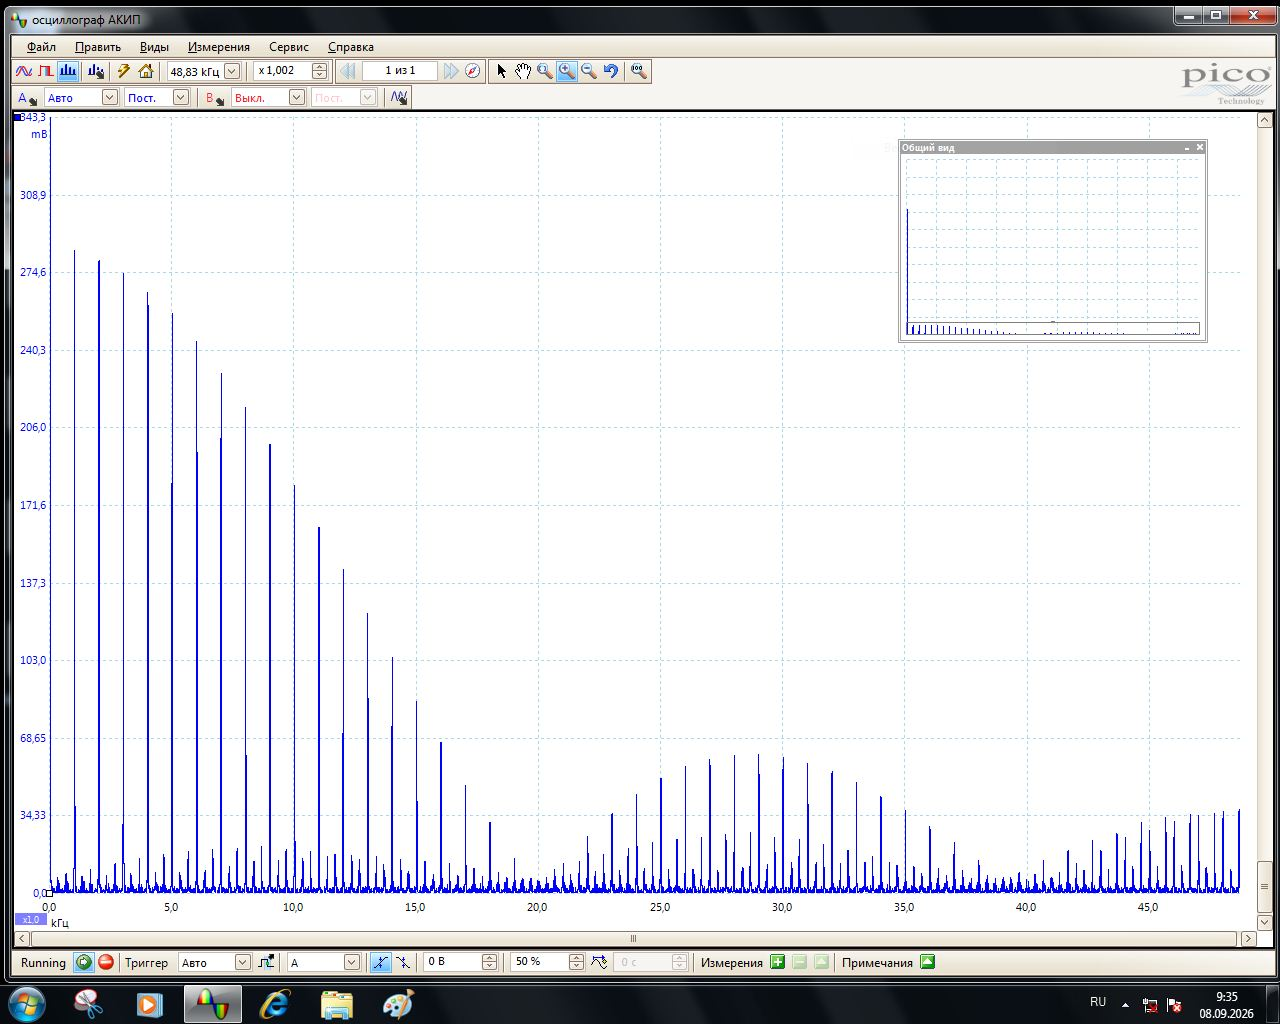
\includegraphics[width=0.7\linewidth]{1}
			\caption{Спектр прямоугольных импульсов $\nu_r = 1\ кГц, \tau = 50 \ мкс$}
			\label{fig:1}
		\end{figure}
		
		При увеличении частоты увеличивалось расстояние между гармониками $\delta \nu$ и росли соответствующее амплитуды, а при увеличении длительности импульса уменьшалась характерная ширина спектра $\Delta \nu$ и так же росла амплитуда. 
		
		
		\begin{figure}[h!]
			\centering
			\subfigure[График $\Delta \nu (\tau^{-1})$]{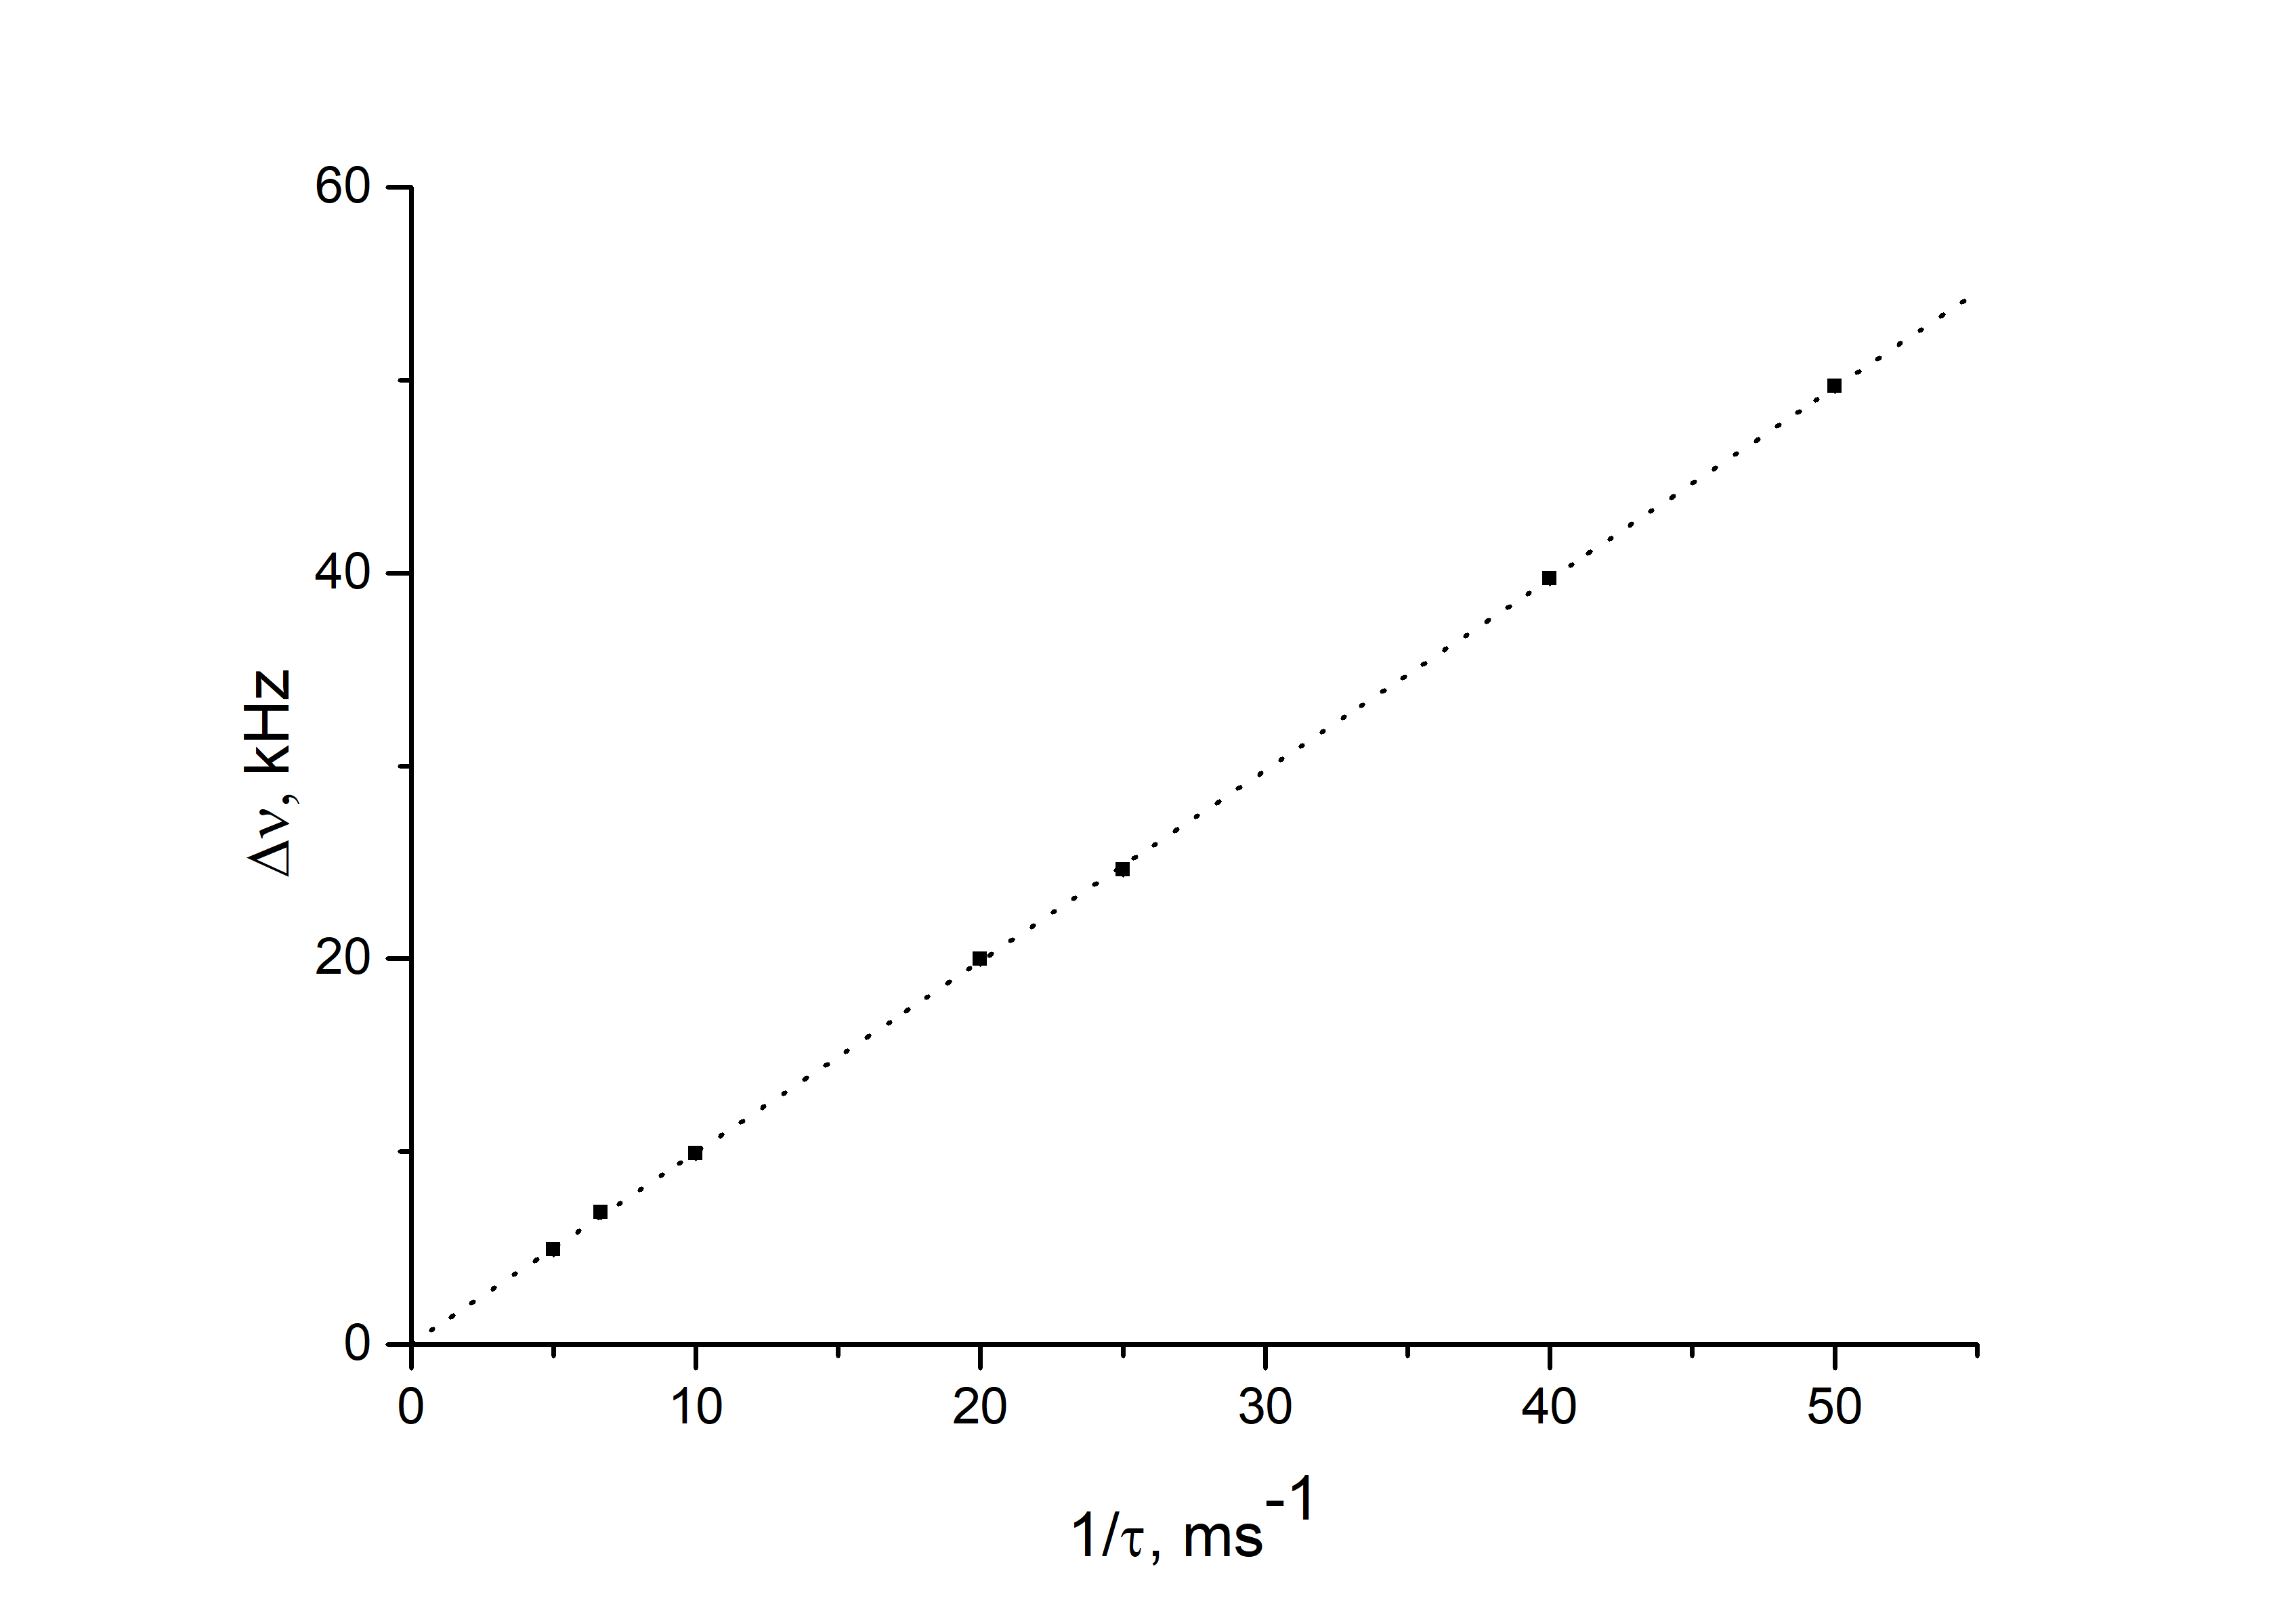
\includegraphics[width=0.49\linewidth]{p8}}
			\subfigure[График $\delta \nu (T^{-1})$]{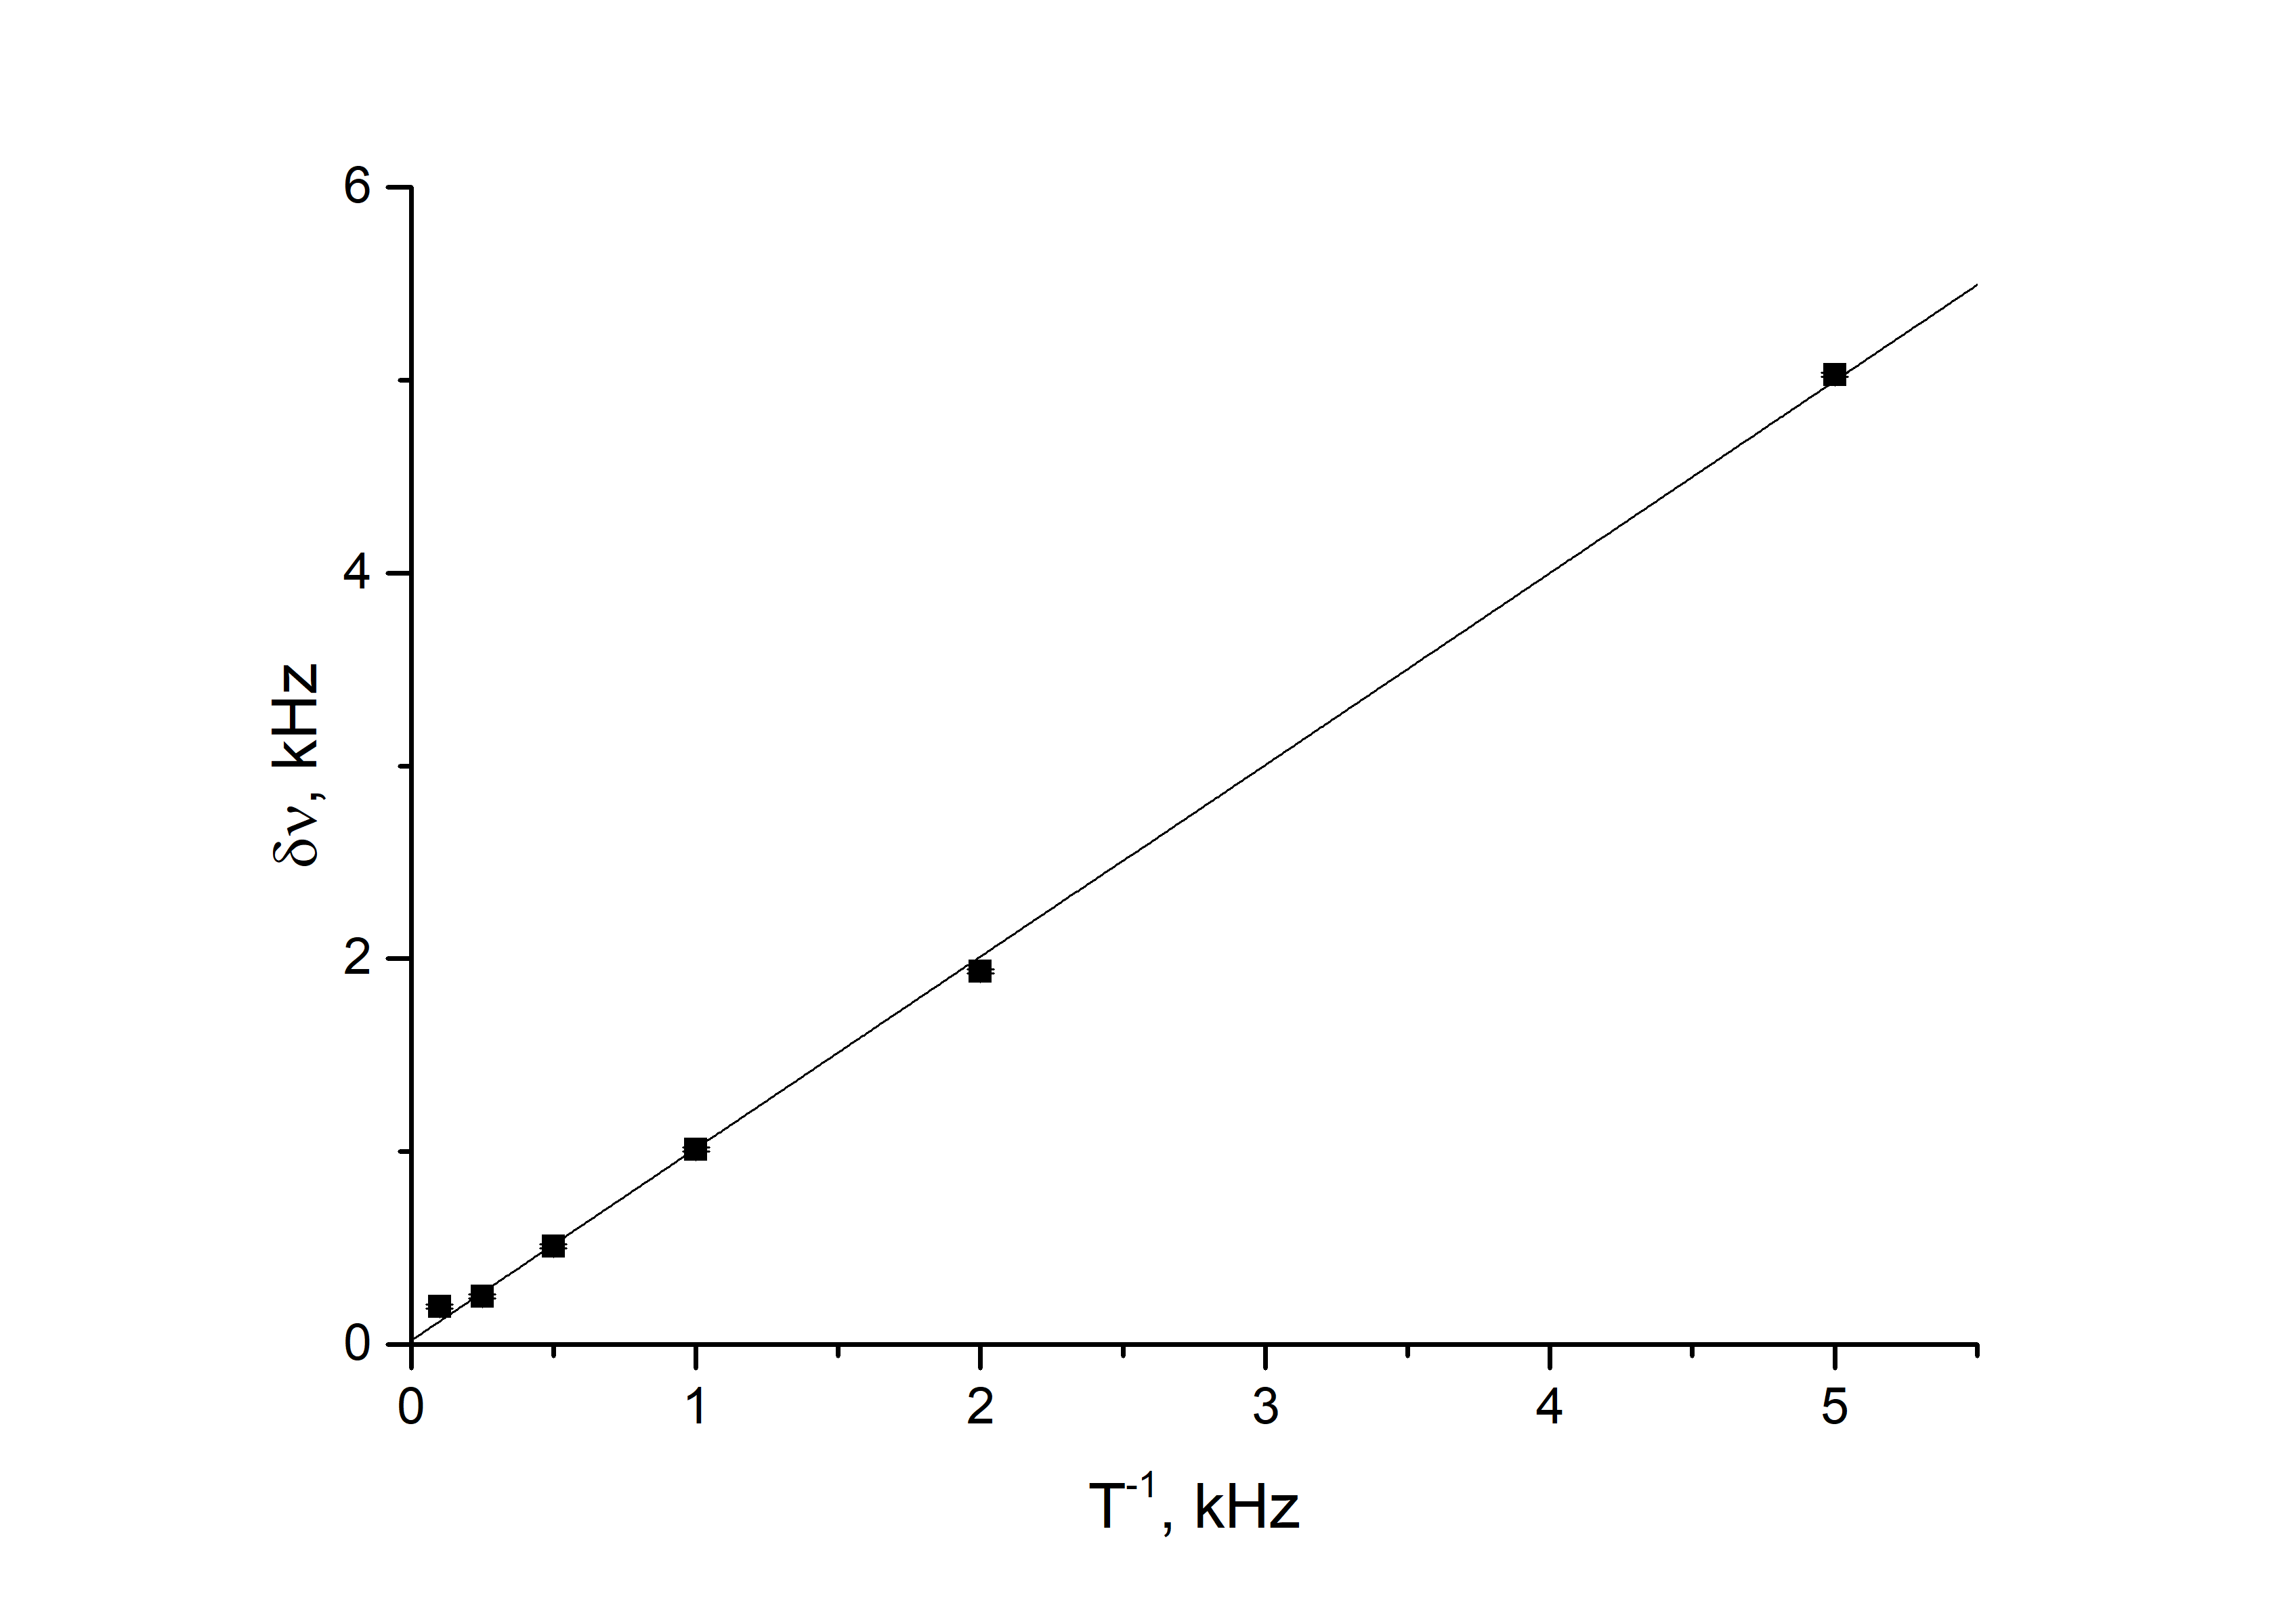
\includegraphics[width=0.49\linewidth]{p9}}
			\caption{}
			\label{fig:plots1}
		\end{figure}
		
		
		Сняты зависимости $\Delta \nu (\tau)$ и $\delta \nu (T)$ , построены графики $\Delta \nu (\tau^{-1})$ и  $\delta \nu (T^{-1})$ (см. рис. \ref{fig:plots1}), по методу наименьших квадратов определены угловые коэффициенты этих зависимостей
		
		\[k_1 = 0,991 \pm 0,003 \ \ \ k_2 = 0,995 \pm 0,014 \]
		
		что подтверждает справедливость соотношения неопределённости.

		
		
	
	
	
	\subsection{Периодические цуги}
	
	На генераторе был установлен режим периодических импульсов синусоидальной формы (цугов) с частотой несущей $\nu_0 = 50 \ кГц$, периодом повторения $T = 1\ мс$, числом периодов синусоиды в импульсе $N = 5$. 
	
	\begin{figure}[h!]
		\centering
		\subfigure[$\nu_0 = 50\ кГц, T = 1 \ мс, \ N = 5$]{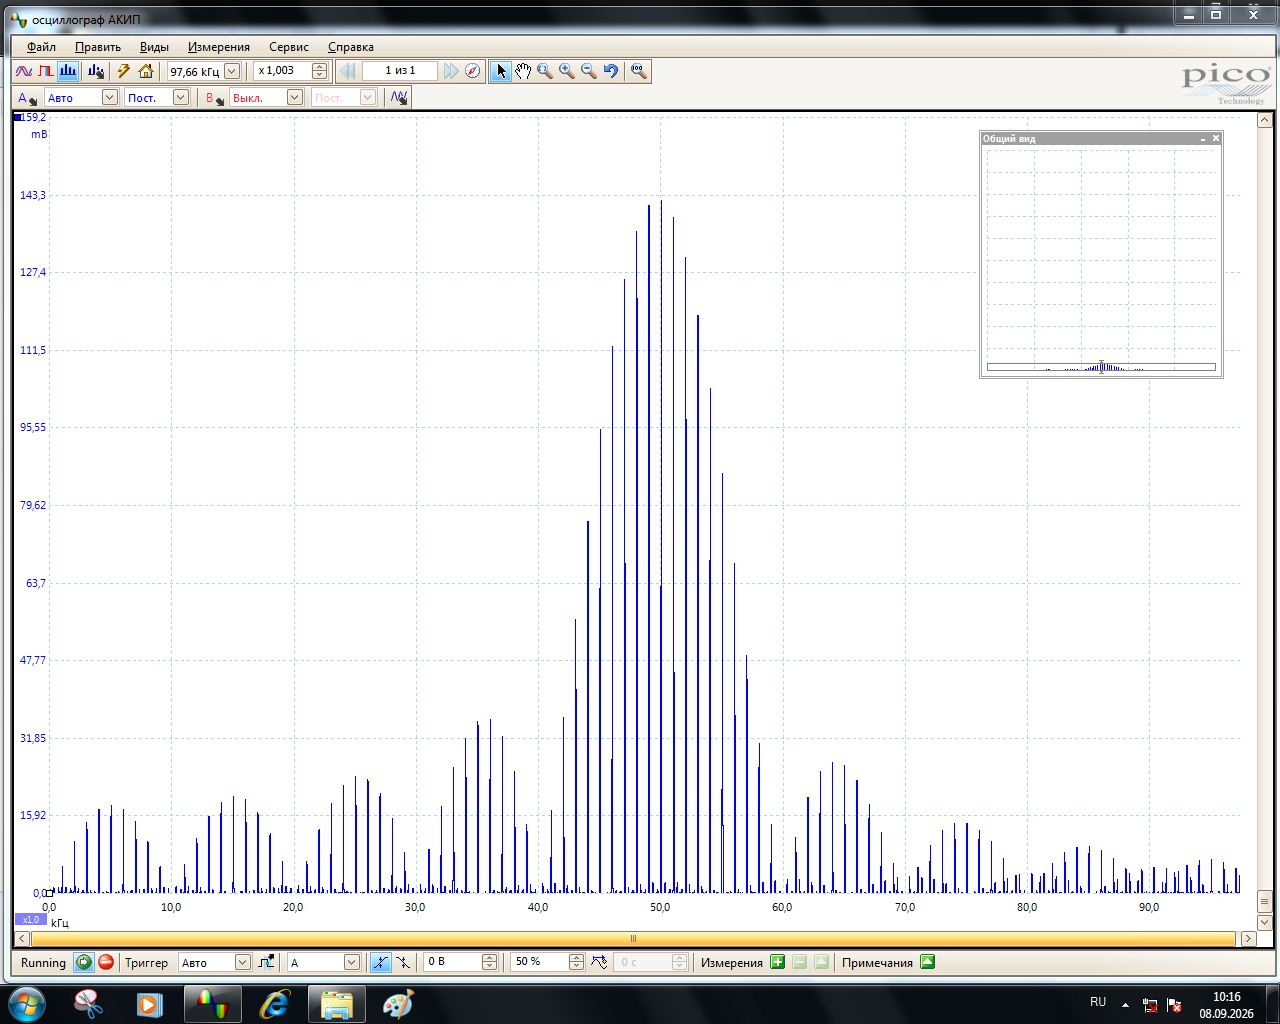
\includegraphics[width=0.45\linewidth]{15}}
		\subfigure[$\nu_0 = 50\ кГц, T = 1 \ мс, \ N = 10$]{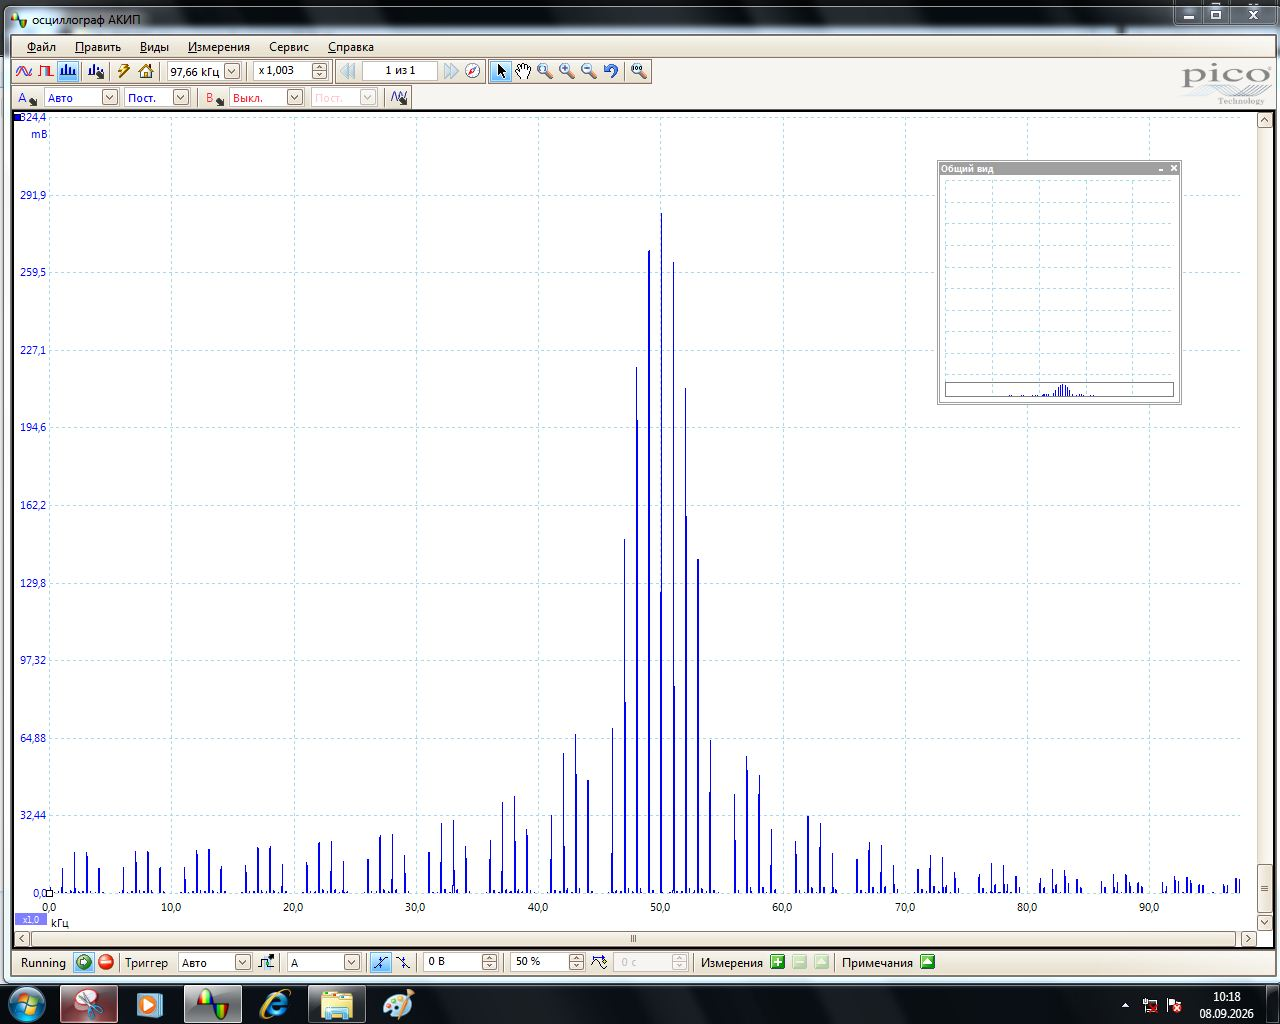
\includegraphics[width=0.45\linewidth]{16}}
		\subfigure[$\nu_0 = 30\ кГц, T = 1 \ мс, \ N = 5$]{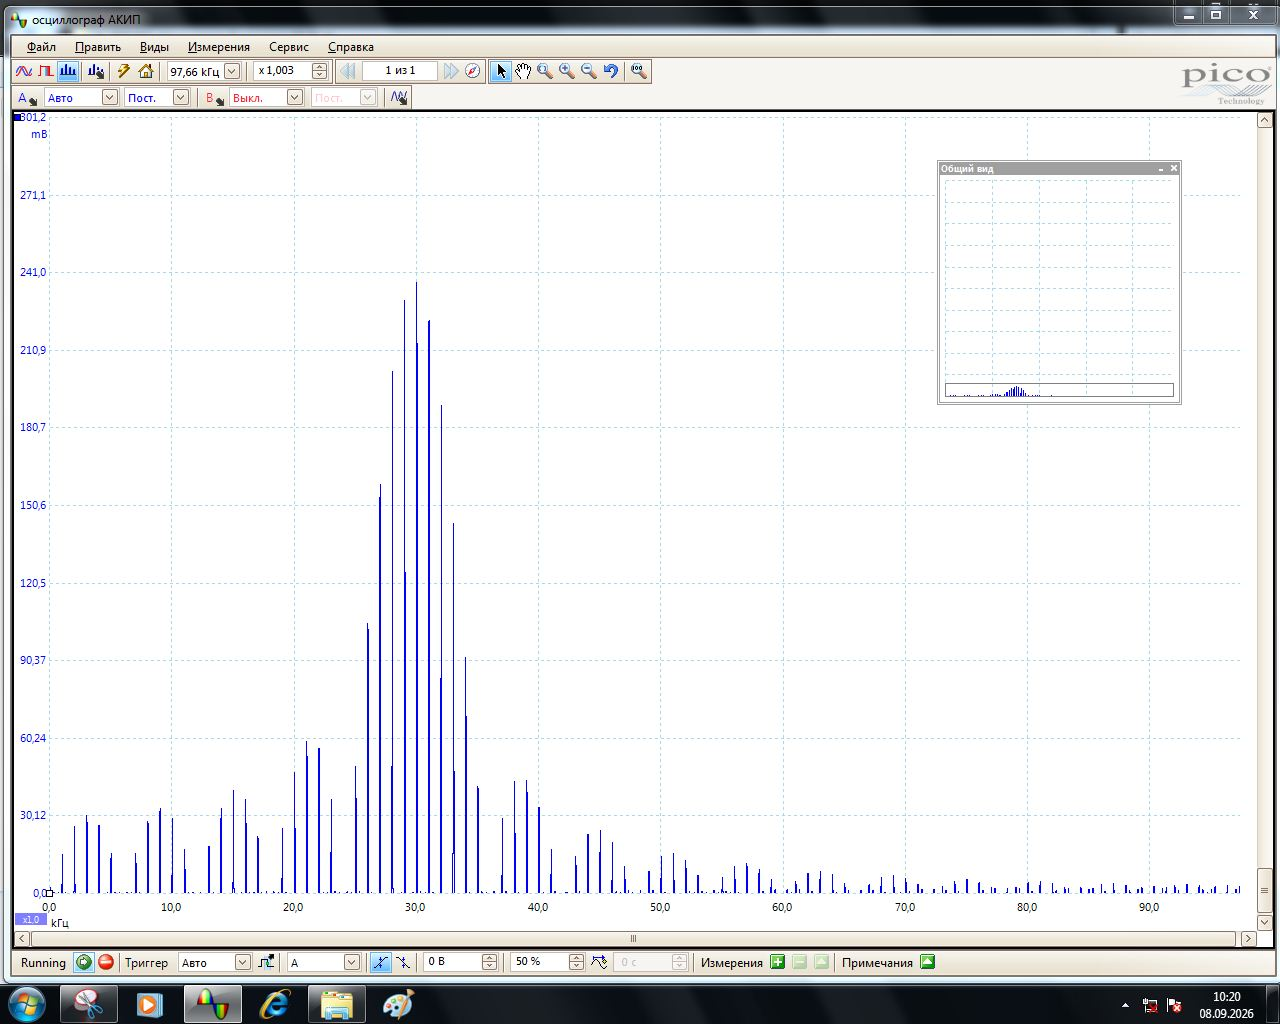
\includegraphics[width=0.45\linewidth]{19}}
		\subfigure[$\nu_0 = 50\ кГц, T = 2 \ мс, \ N = 5$]{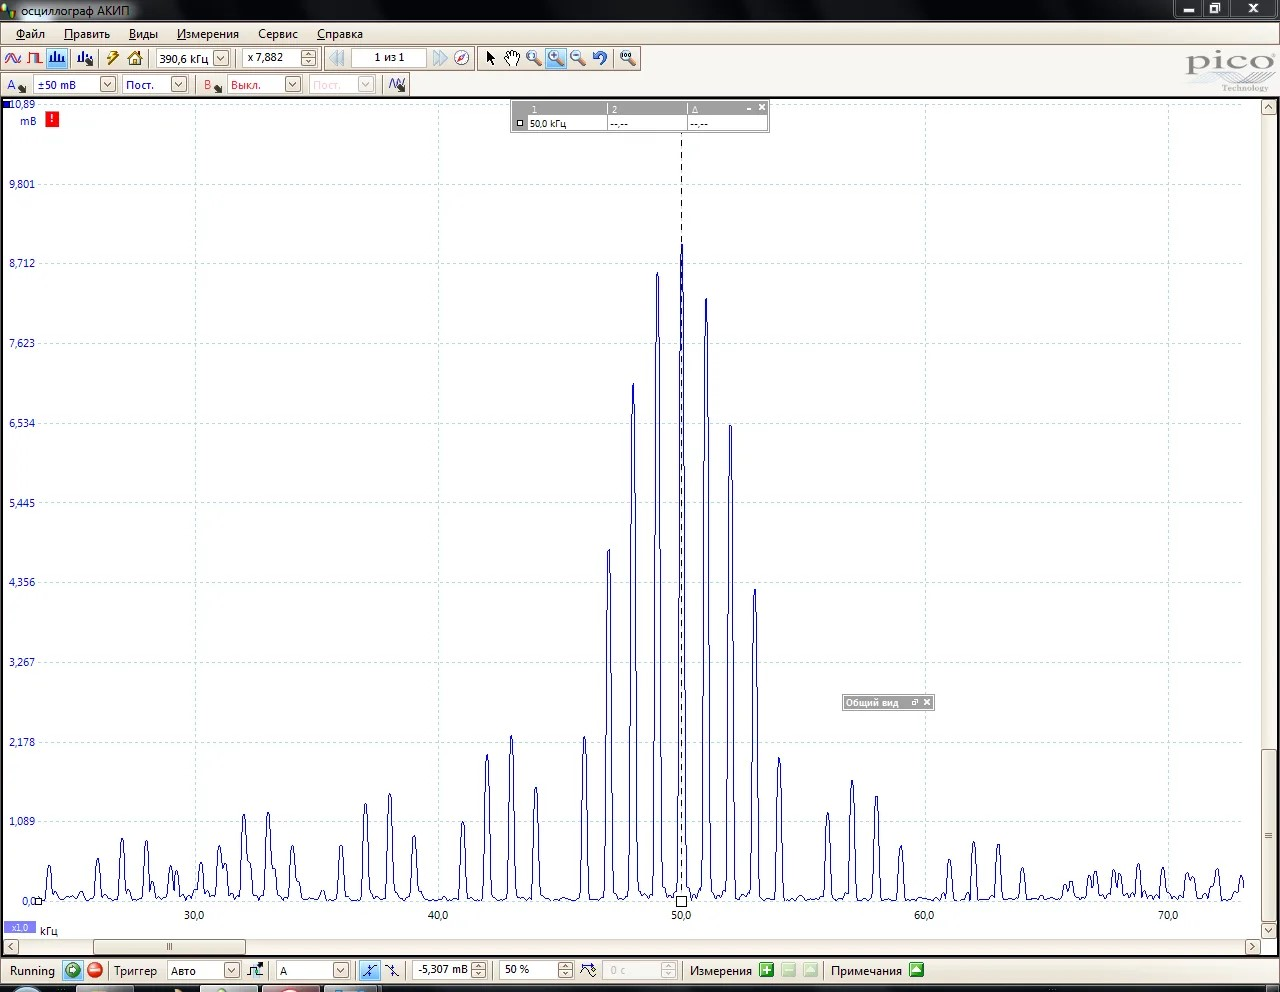
\includegraphics[width=0.45\linewidth]{M}}
		\caption{Спектры цугов}
		\label{fig:s2}
	\end{figure}
	
	Увеличение T до 2 мс уменьшило расстояние между гармониками примерно от 1 до 0,5 кГц.
	Увеличение N до 10 уменьшило
	ширину спектра примерно в 2 раза. Увеличение несущей до 75 кГц
	сместило спектр и увеличило ширину спектра примерно до 30 кГц.
	Измеренные по шкалам положения минимумов и частотные интервалы собраны в табл. 5. Таким образом, подтверждена справедливость соотношения неопределённостей.
	
	
	\subsection{Амплитудная модуляция}
	
	На генераторе был установлен режим амплитудной модуляции синусоидального сигнала с параметрами: частота несущей $\nu_0 = 50\ кГц$, частота модуляции $\nu_m = 2\ кГц$, глубина модуляции $m = 0,5$ (см. рис. \ref{fig:am}).
	
	\begin{figure}[h!]
		\centering
		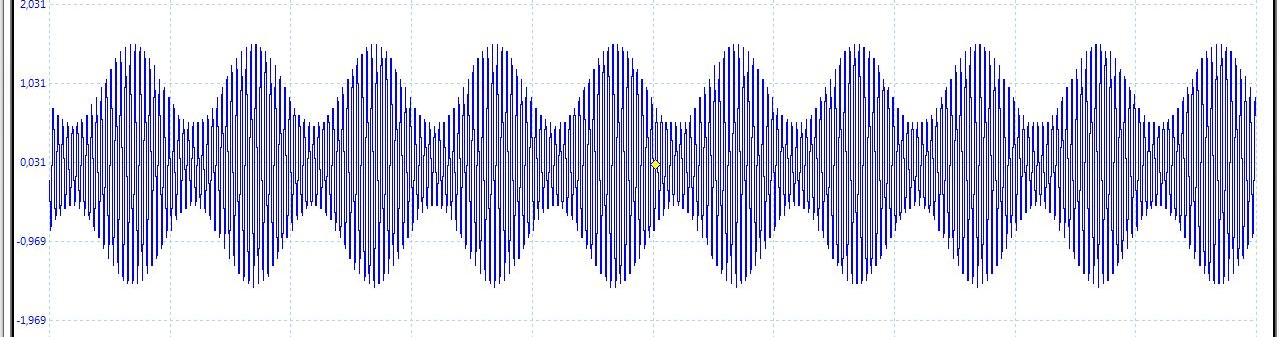
\includegraphics[width=1\linewidth]{67}
		\caption{График амлитудно-модулированного сигнала на осциллографе}
		\label{fig:am}
	\end{figure}
	
	Максимальная и минимальная амплитуды сигнала составили $A_{max}=(1,521 \pm 0,001) \ усл.ед.; \ A_{min}=(0,498\pm 0,001) \ усл.ед.$. Рассчитанная по ним глубина модуляции $\tilde{m} =(0,51 \pm 0,01)$, что соответствует заданной глубине модуляции. Заметим, что максимальная и минимальная амплитуда не независимы, поэтому для оценки погрешности принята корреляция, равная 1.
	
	На полученном спектре амплитудно-модулированного сигнала имеется одна основная спектральная линия и две боковые (см. рис. \ref{fig:amsp}). 

	\begin{figure}[h!]
		\centering
		\subfigure[$\nu_0 = 50\ кГц, \nu_m = 2\ кГц,  m = 0,5$]{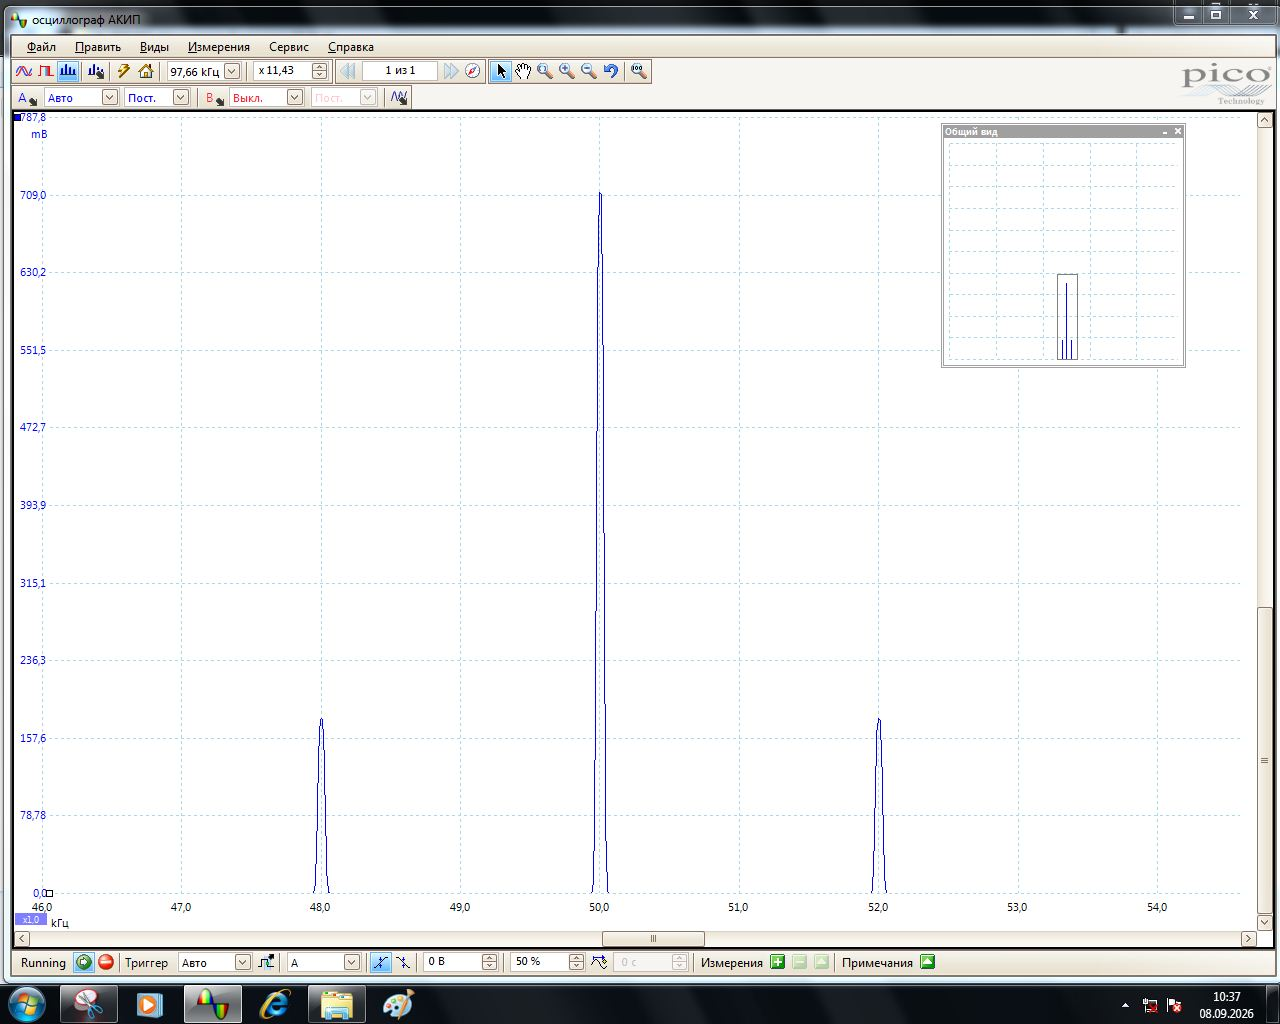
\includegraphics[width=0.45\linewidth]{22}}
		\subfigure[$\nu_0 = 30\ кГц, \nu_m = 2\ кГц,  m = 0,5$]{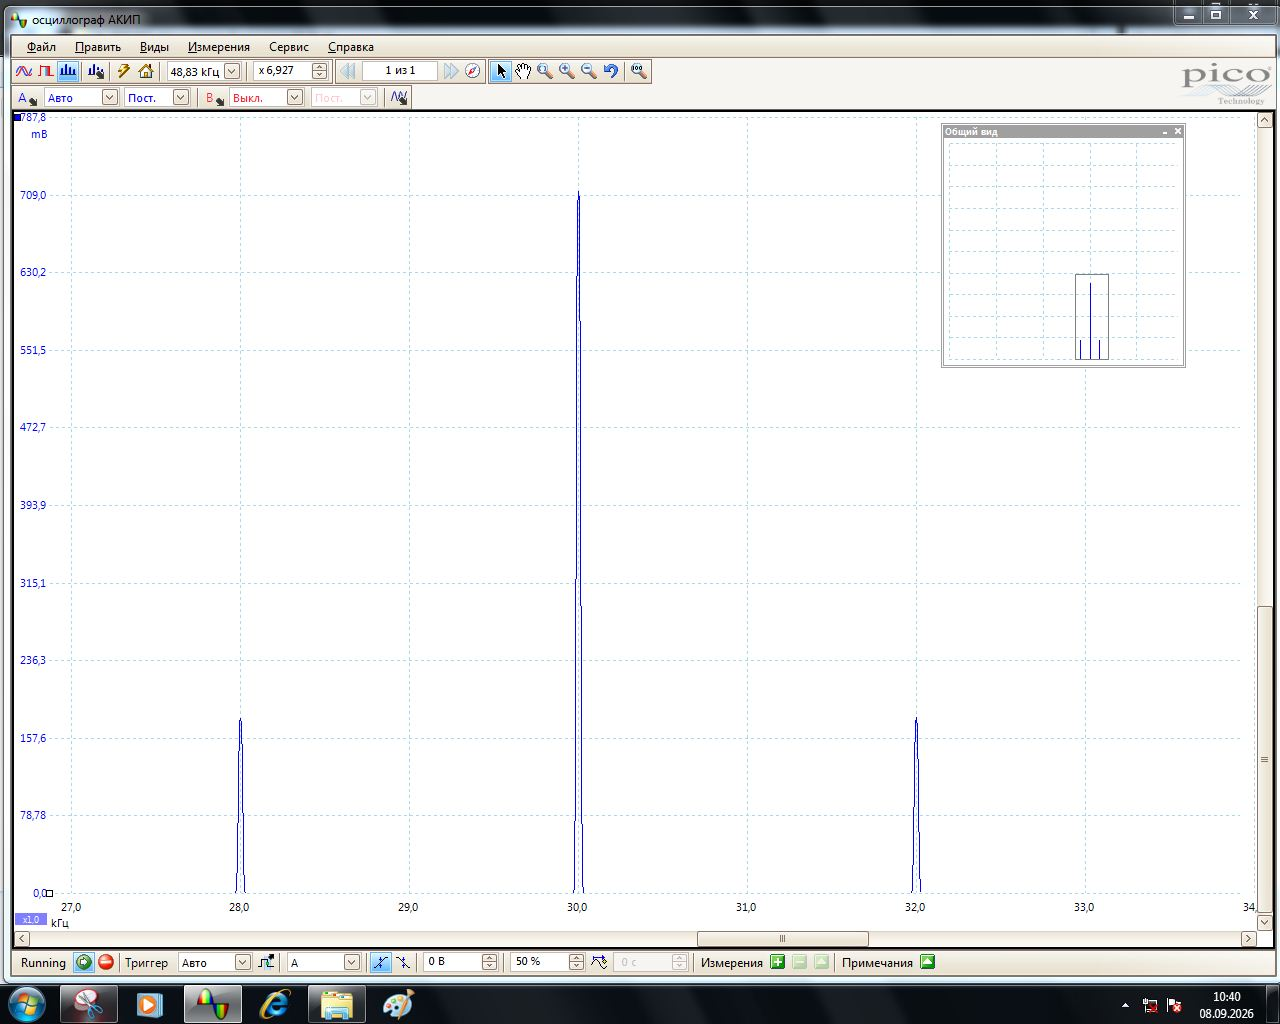
\includegraphics[width=0.45\linewidth]{23}}
		\subfigure[$\nu_0 = 50\ кГц, \nu_m = 4\ кГц,  m = 0,5$]{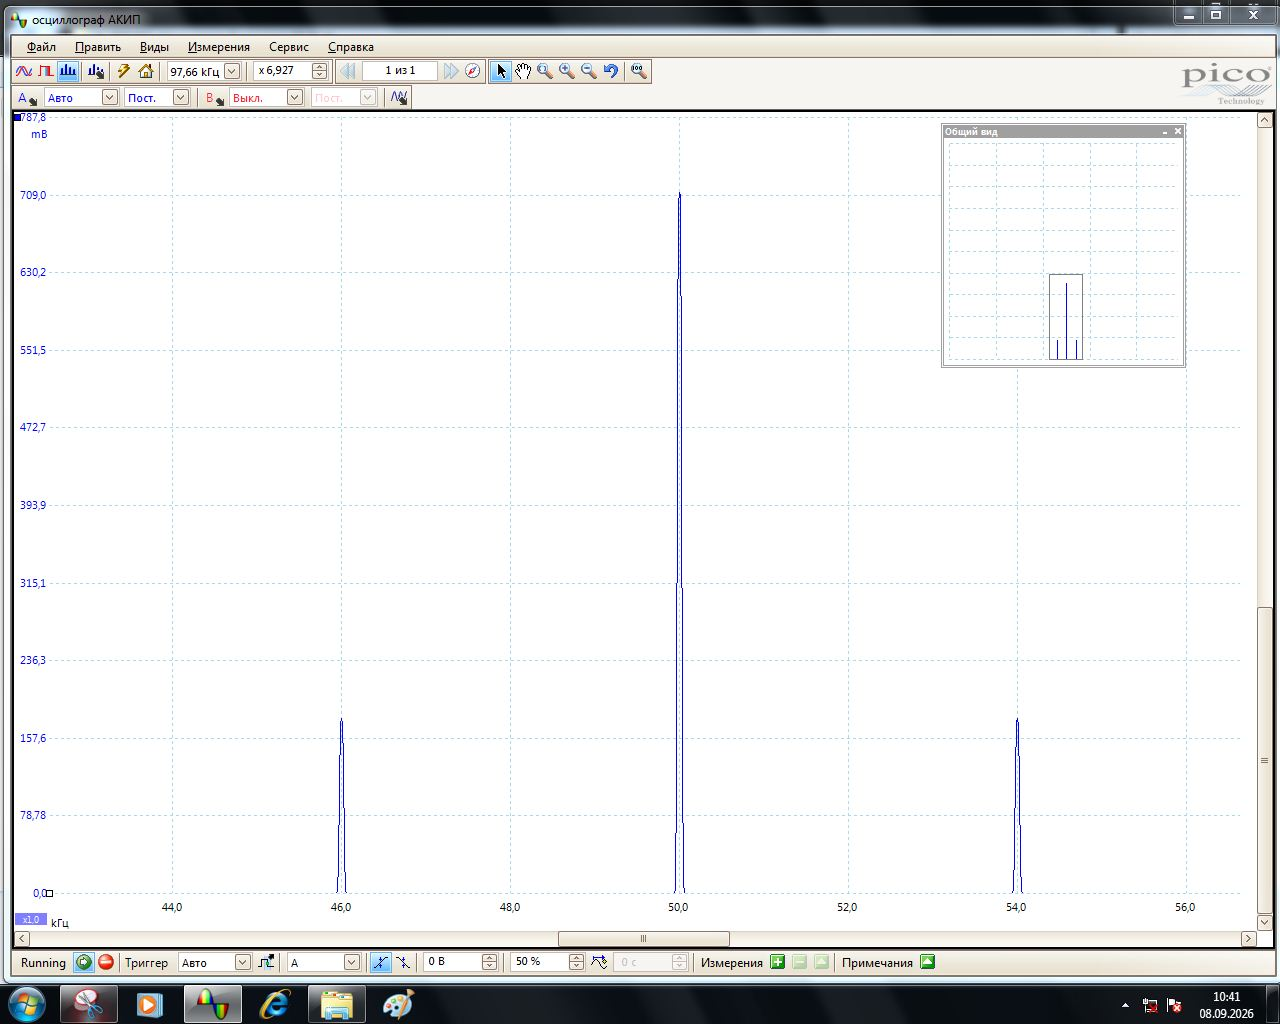
\includegraphics[width=0.45\linewidth]{24}}
		\subfigure[$\nu_0 = 50\ кГц, \nu_m = 2\ кГц,  m = 0,1$]{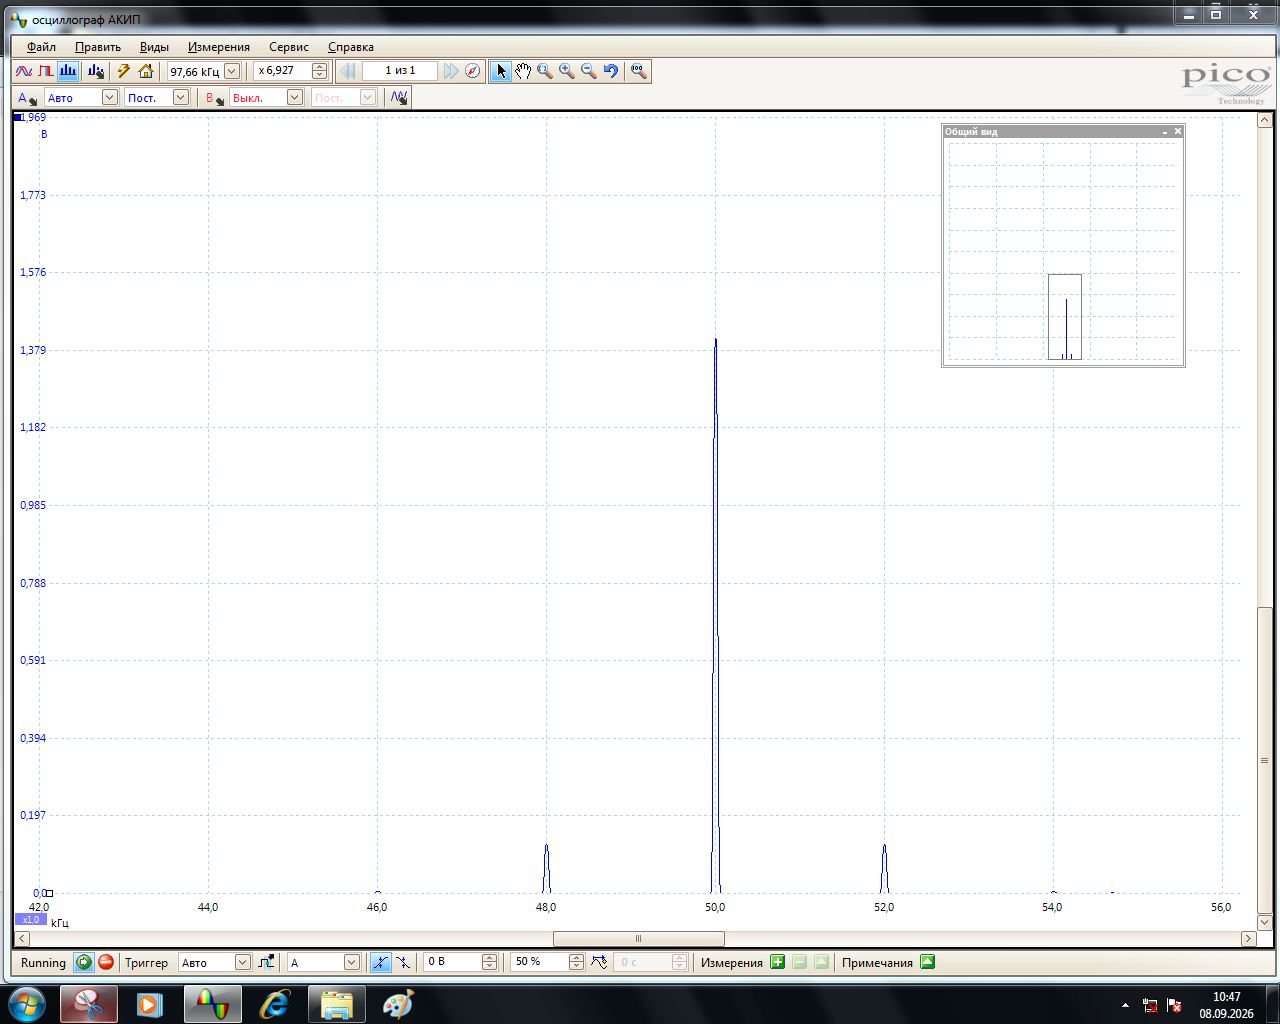
\includegraphics[width=0.45\linewidth]{25}}
		\caption{Спектры амплитудно-модулированных сигналов}
		\label{fig:amsp}
	\end{figure}
	
	При изменении несущей частоты соответственно сдвигается спектр, а при изменении модулирующей -- расстояние между гармониками. Глубина модуляции влияет на высоту боковых пиков.
	
	\begin{figure}[h!]
		\centering
		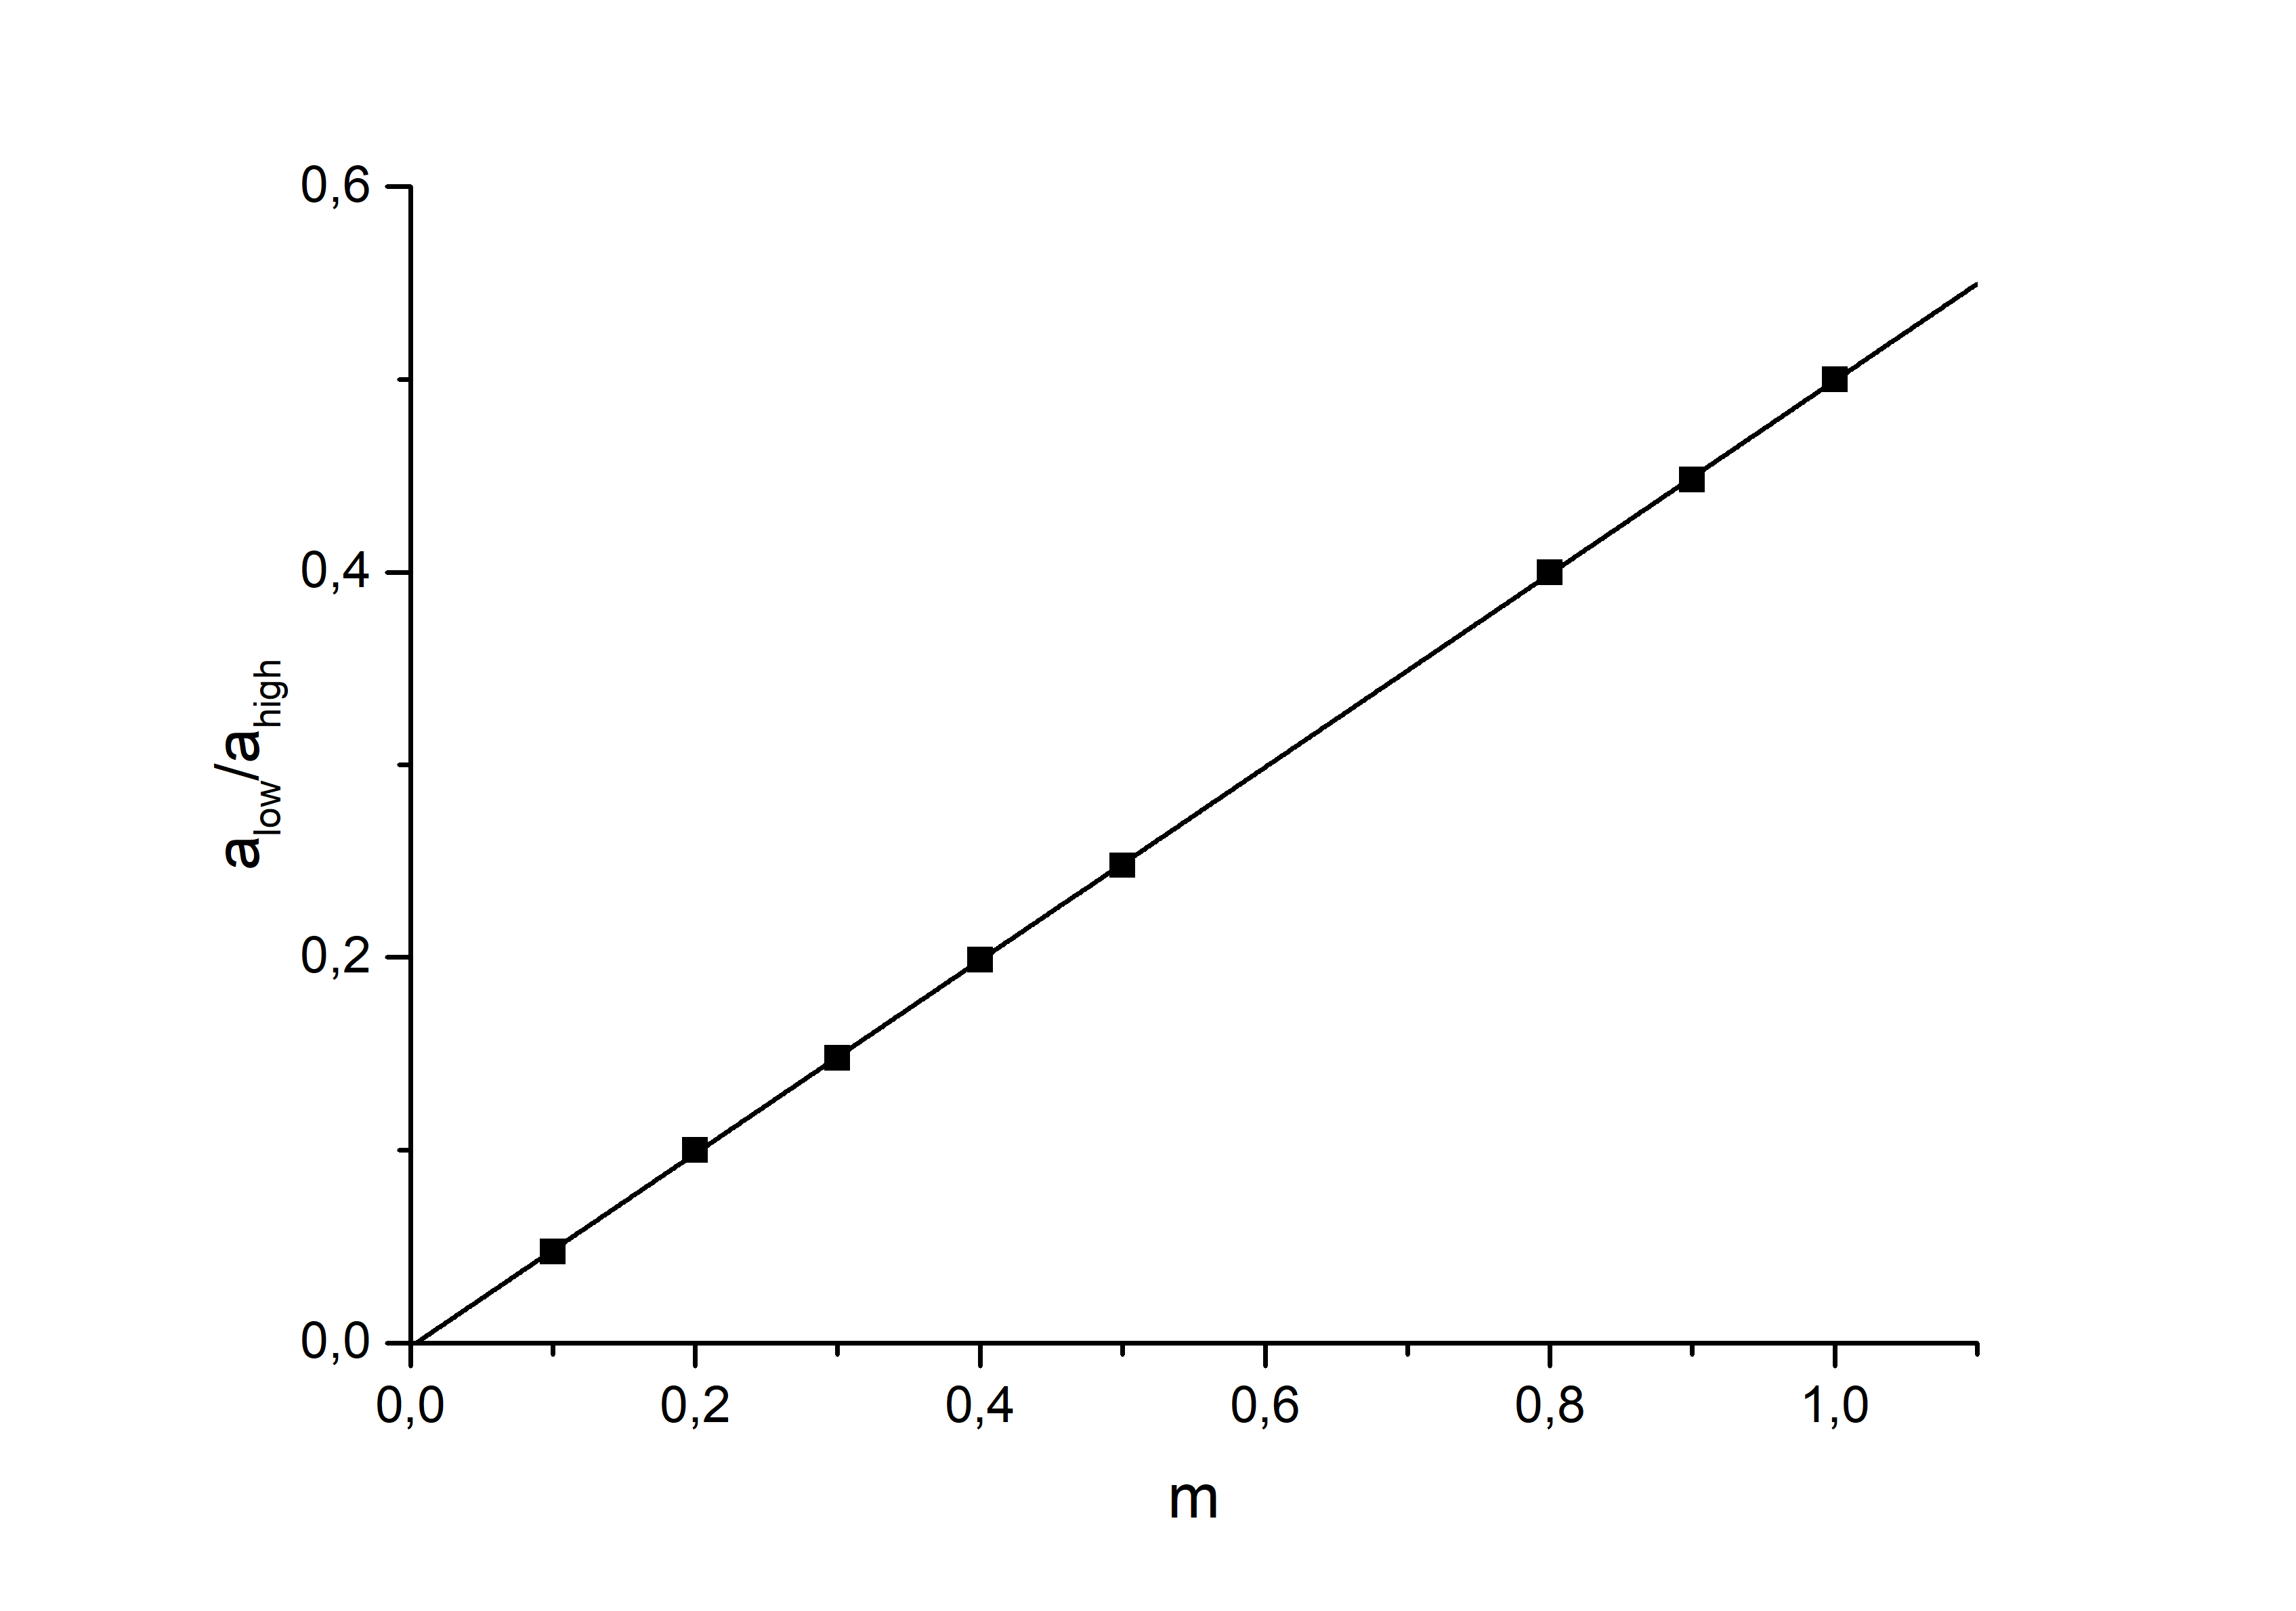
\includegraphics[width=0.7\linewidth]{p23}
		\caption{График зависимости $a_{бок}/a_{осн}(m)$}
		\label{fig:ampl}
	\end{figure}
	
	
	По угловому коэффициенту графика зависимости $a_{бок}/a_{осн}(m)$ (см. рис. \ref{fig:ampl}) -- $k_m = 0,5014 \pm 0,0013$  показано, что 
	
	\[a_{бок} =\frac{ ma_{осн}}{2} \] 
	
	\begin{figure}[h!]
	\centering
	\subfigure[$\nu_0 = 50\ кГц, \nu_m = 2\ кГц,  \phi_m = 30^o$]{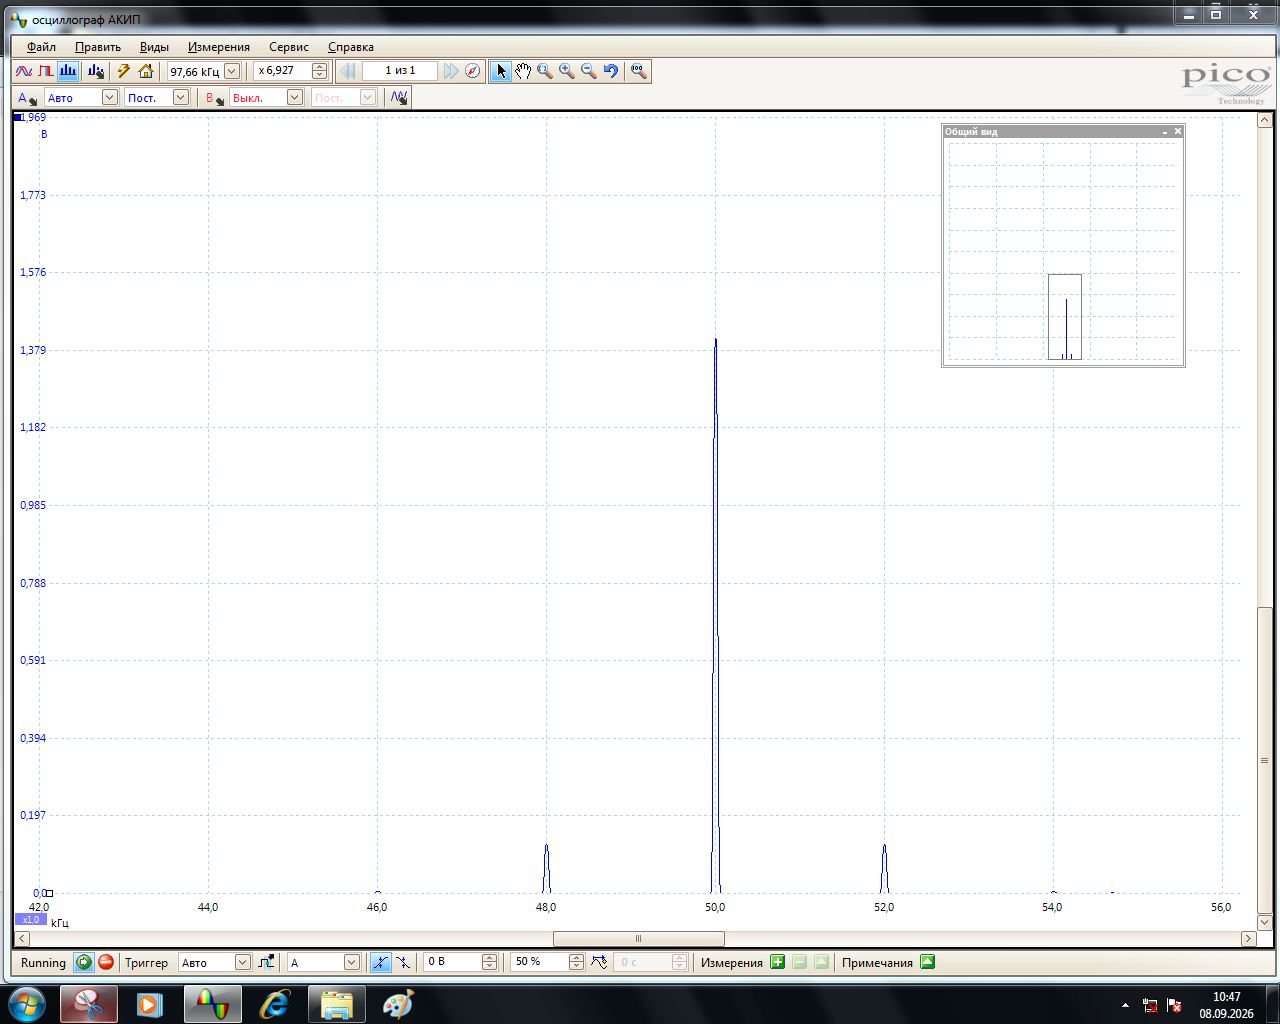
\includegraphics[width=0.45\linewidth]{25}}
	\subfigure[$\nu_0 = 50\ кГц, \nu_m = 2\ кГц,  \phi_m = 50^o$]{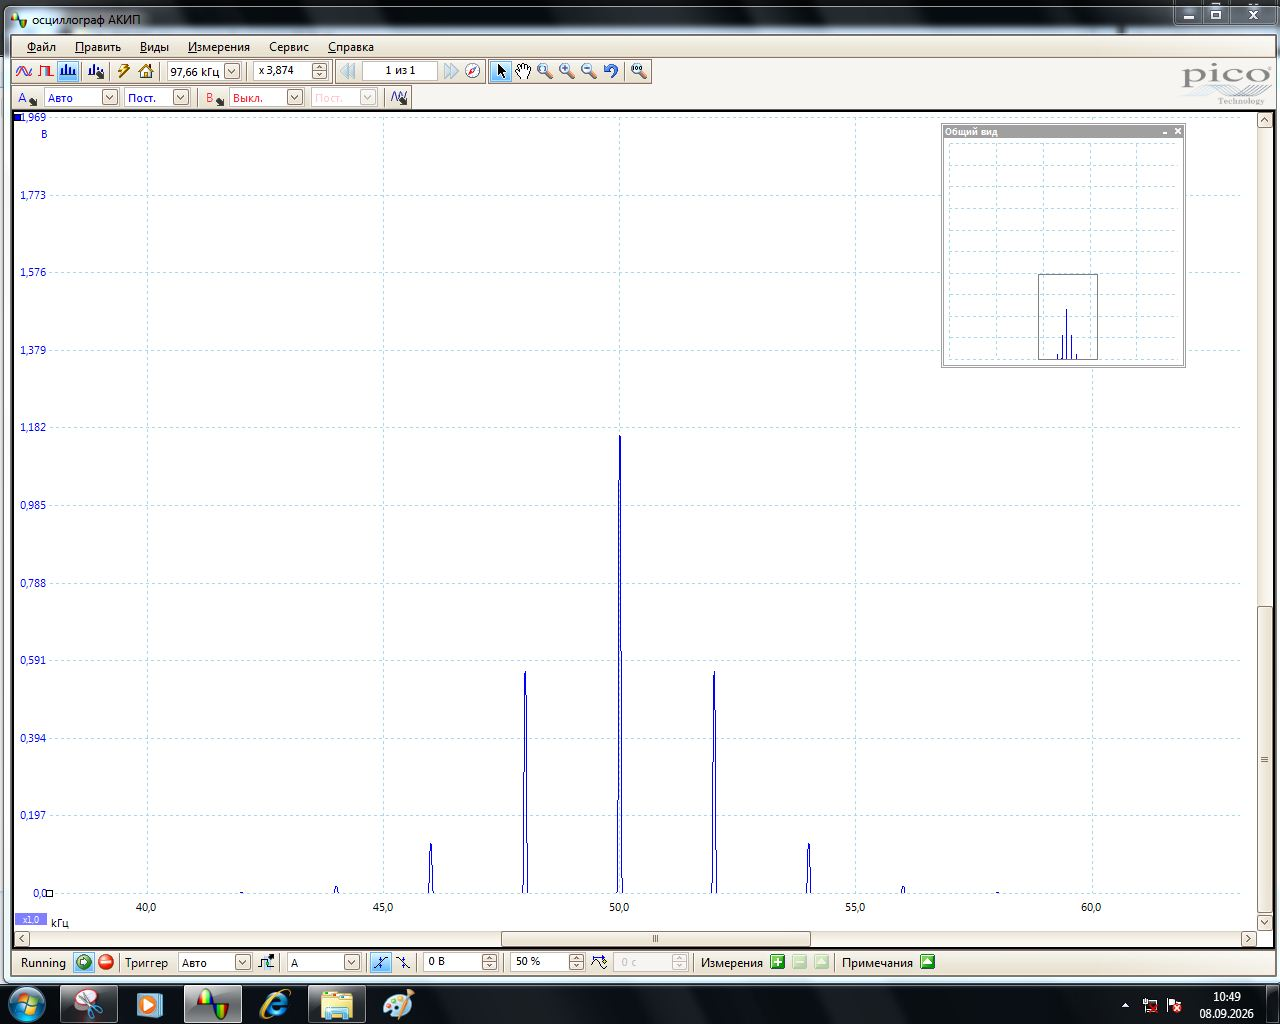
\includegraphics[width=0.45\linewidth]{26}}
	\subfigure[$\nu_0 = 100\ кГц, \nu_m = 2\ кГц,  \phi_m = 30^o$]{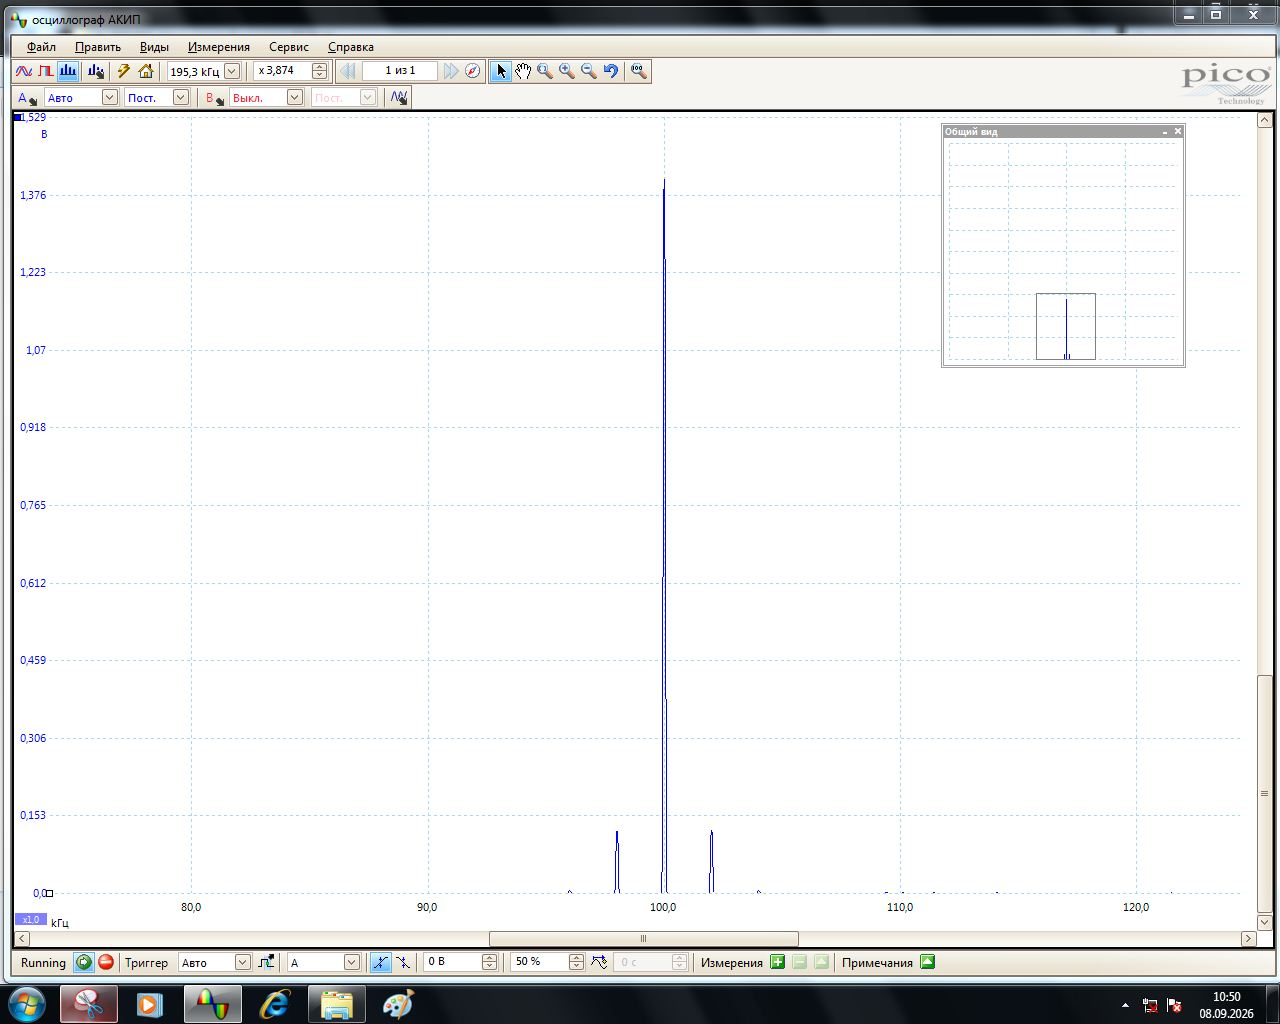
\includegraphics[width=0.45\linewidth]{27}}
	\subfigure[$\nu_0 = 50\ кГц, \nu_m = 10\ кГц,  \phi_m = 30^o$]{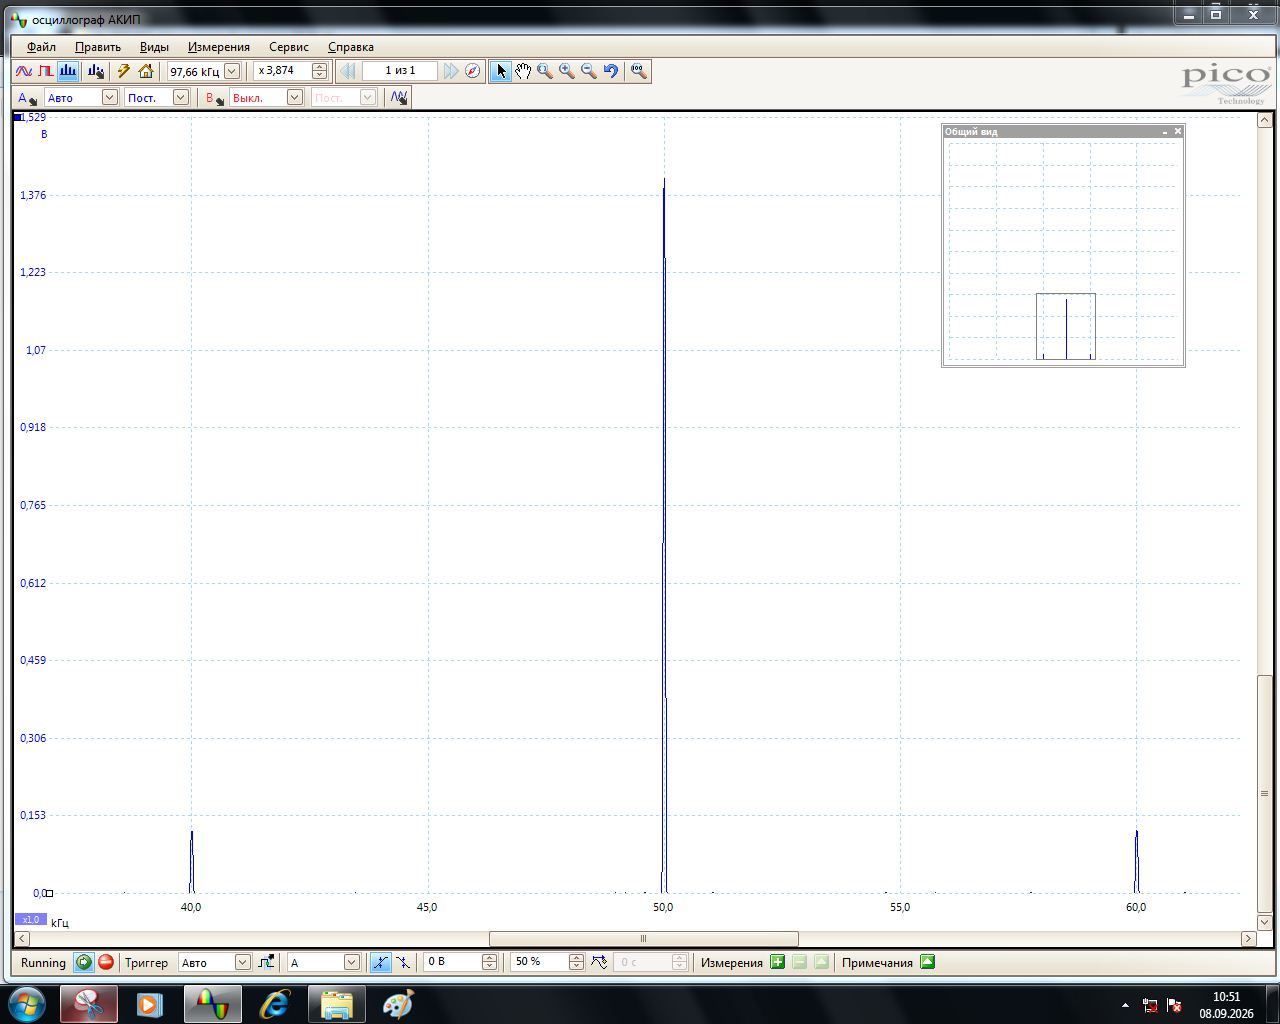
\includegraphics[width=0.45\linewidth]{28}}
	\caption{Спектры фазово-модулированных сигналов}
	\label{fig:fmsp}
\end{figure}	
	
	\subsection{Фазовая модуляция}
	
	На генераторе был установлен режим фазовой модуляции синусоидального сигнала с параметрами: частота несущей $\nu_0 = 50\ кГц$, частота модуляции $\nu_m = 2\ кГц$, глубина модуляции $\phi_m = 30^o$.
	

	
	На полученном спектре амплитудно-модулированного сигнала имеется одна основная спектральная линия и две боковые (см. рис. \ref{fig:fmsp}). 
	

	
	При изменении несущей частоты соответственно сдвигается спектр, а при изменении модулирующей -- расстояние между гармониками. Глубина модуляции влияет на высоту боковых пиков и появление следующих гармоник.
	
	В целом, спектр ФМ-сигнала похож на спектр АМ-сигнала с той же несущей и модулирующей частотами. Лишь при увеличении глубины модуляции на спектре ФМ-сигнала появляются вторые и следующие боковые линии, чего на спектре АМ-сигнала не происходит.
	
	Это сходство показывает, что при спектральном анализе электрических сигналов по амплитудам нарушается взаимно-однозначное соответствие спектра и сигнала, т.к. теряется информация о фазе сигнала.
	
	\subsection{RC-фильтр}
	
	На генераторе был установлен режим прямоугольных импульсов с периодом $T = 3 \ мкс$ и длительностью $\tau = 150 нс$ (см. рис. \ref{fig:rc}). Получены спектры сигналов на входе и выходе цепи.
	
	\begin{figure}[h!]
		\centering
		\subfigure{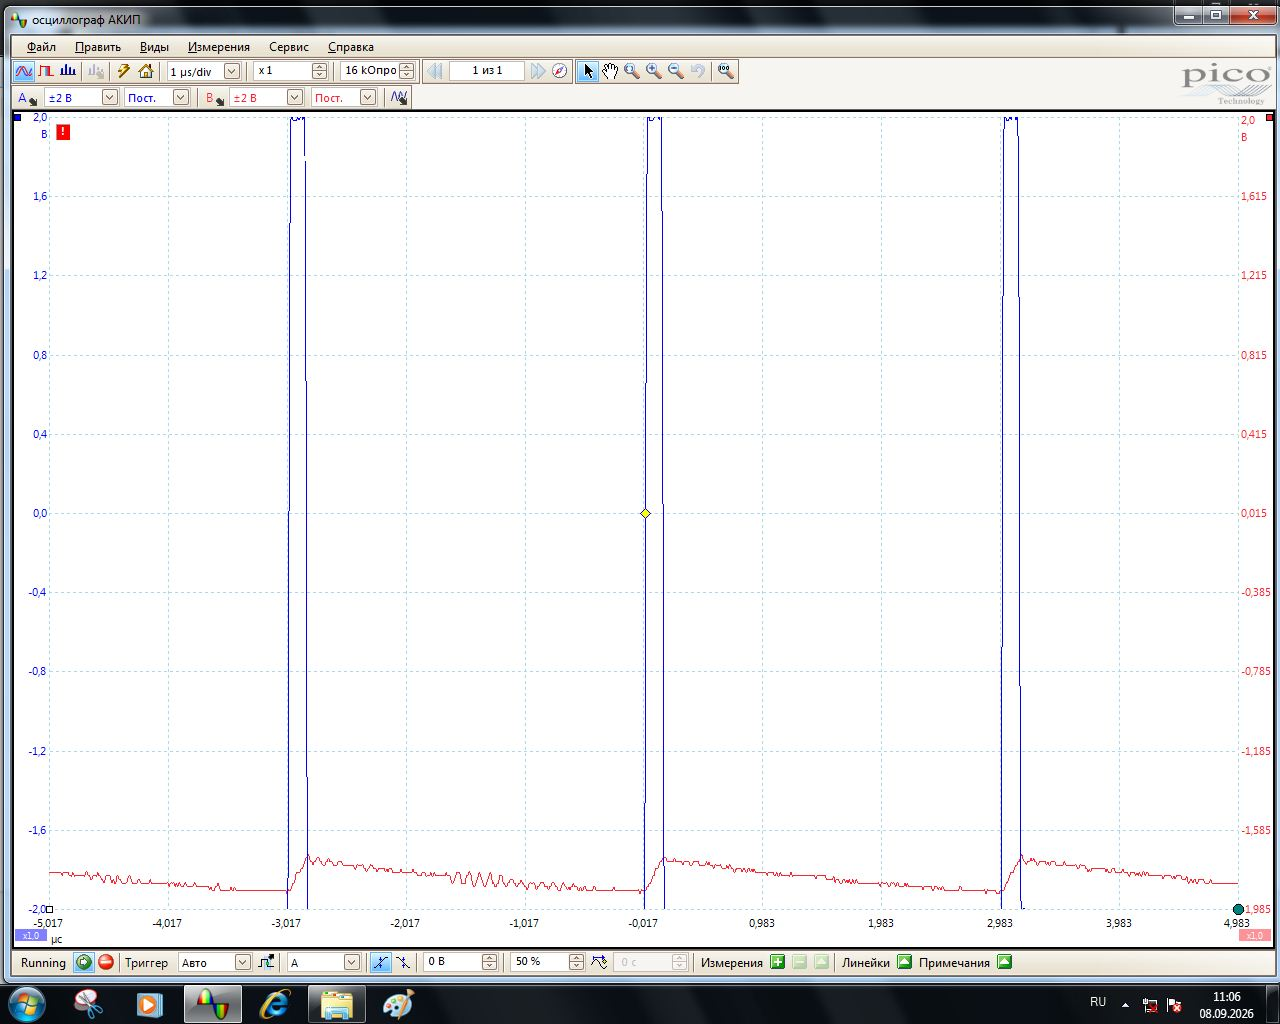
\includegraphics[width=0.45\linewidth]{29}}
		\subfigure{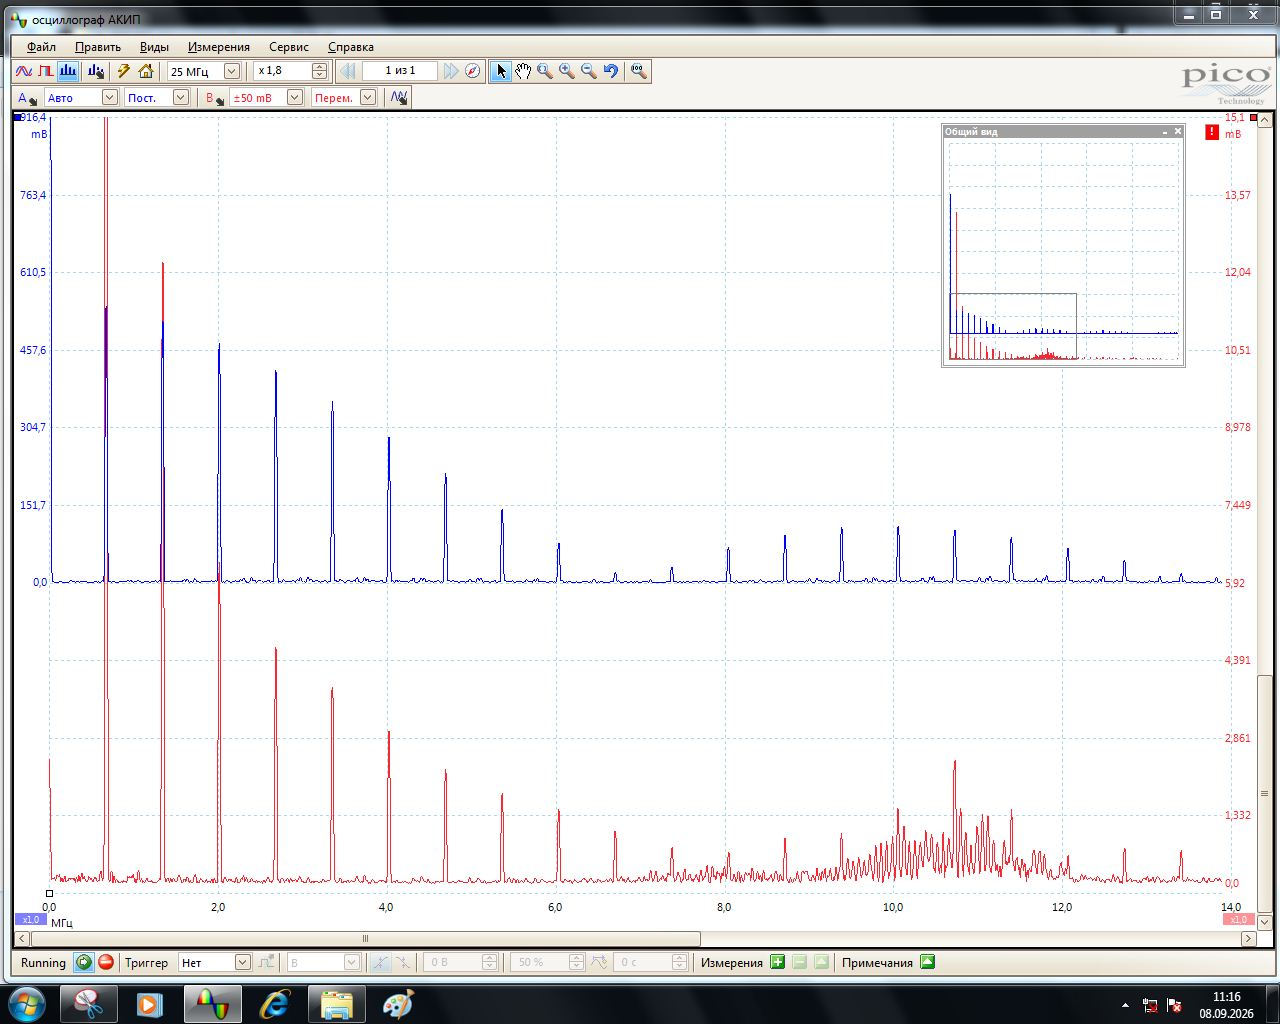
\includegraphics[width=0.45\linewidth]{32}}
		\caption{Графики и спектры сигналов с генератора и выхода RC-цепочки}
		\label{fig:rc}
	\end{figure}
	
	
	По ним проверена зависимость (11) и найдена постоянная времени $\tau = (3,36 \pm 0,11) \ мкс$
	
		\begin{figure}[h!]
		\centering
		\subfigure[График зависимости $K(\nu)$]{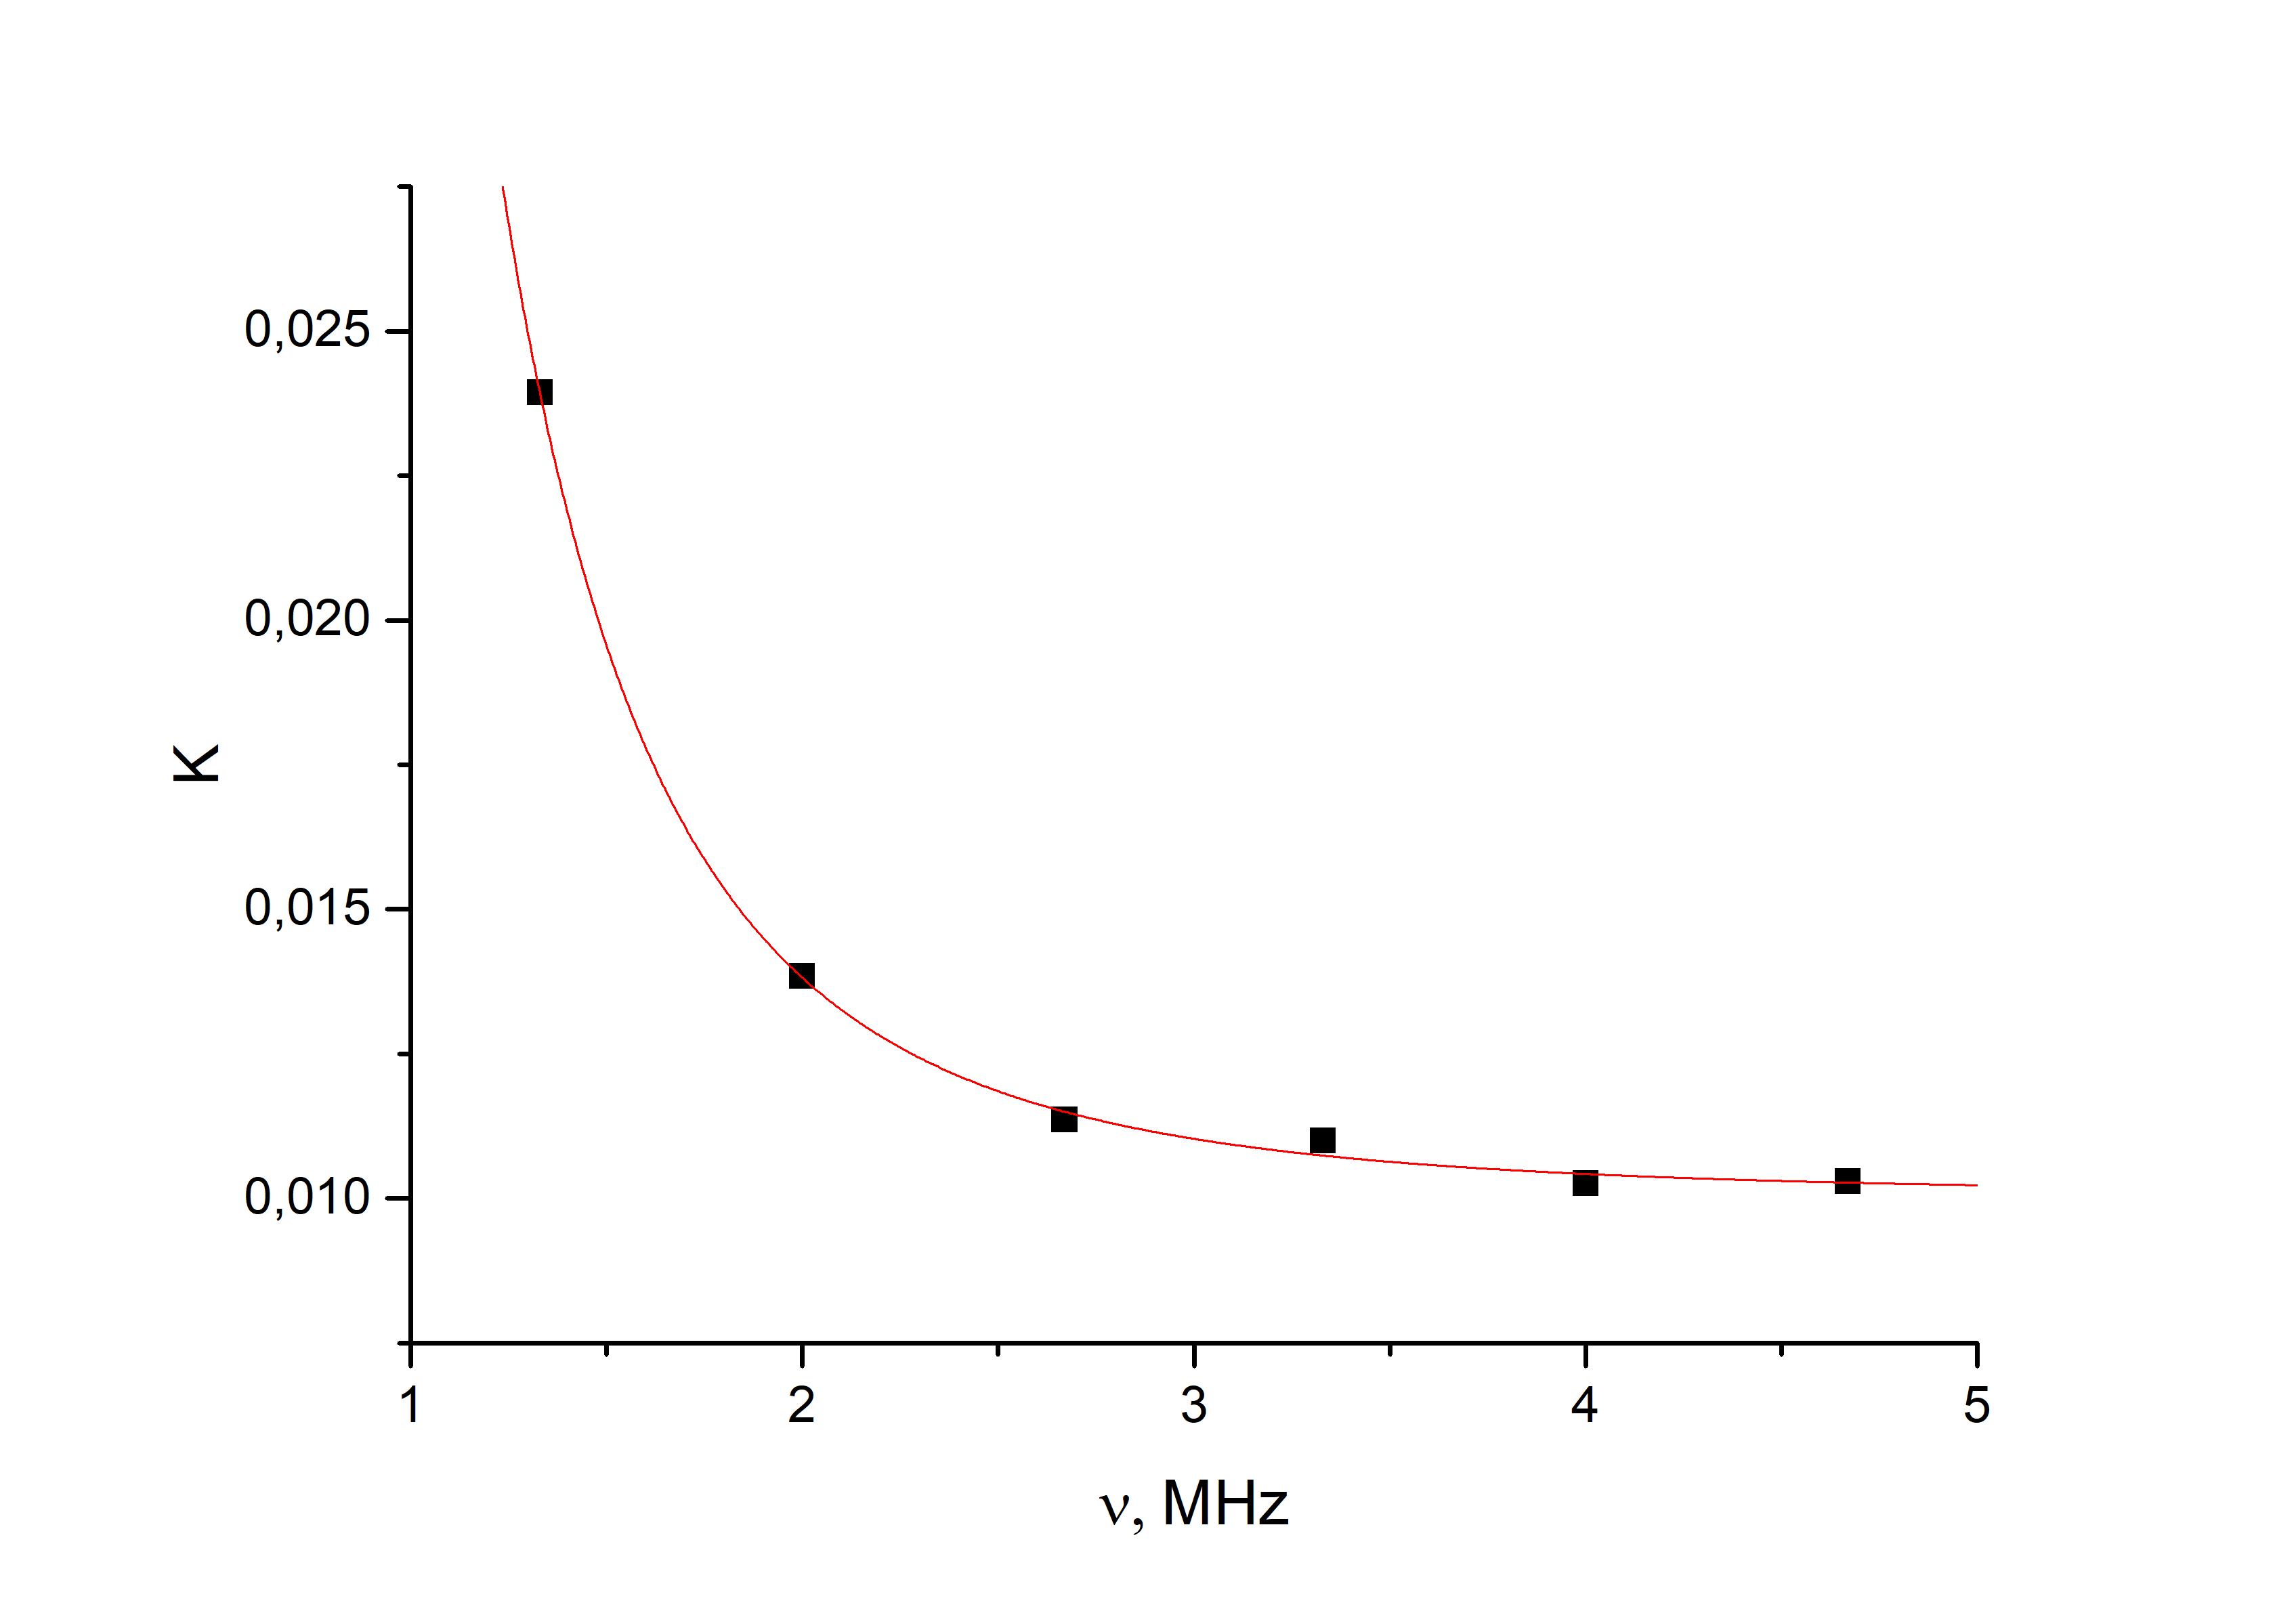
\includegraphics[width=0.45\linewidth]{p29}}
		\subfigure[График зависимости $K(1/\nu)$]{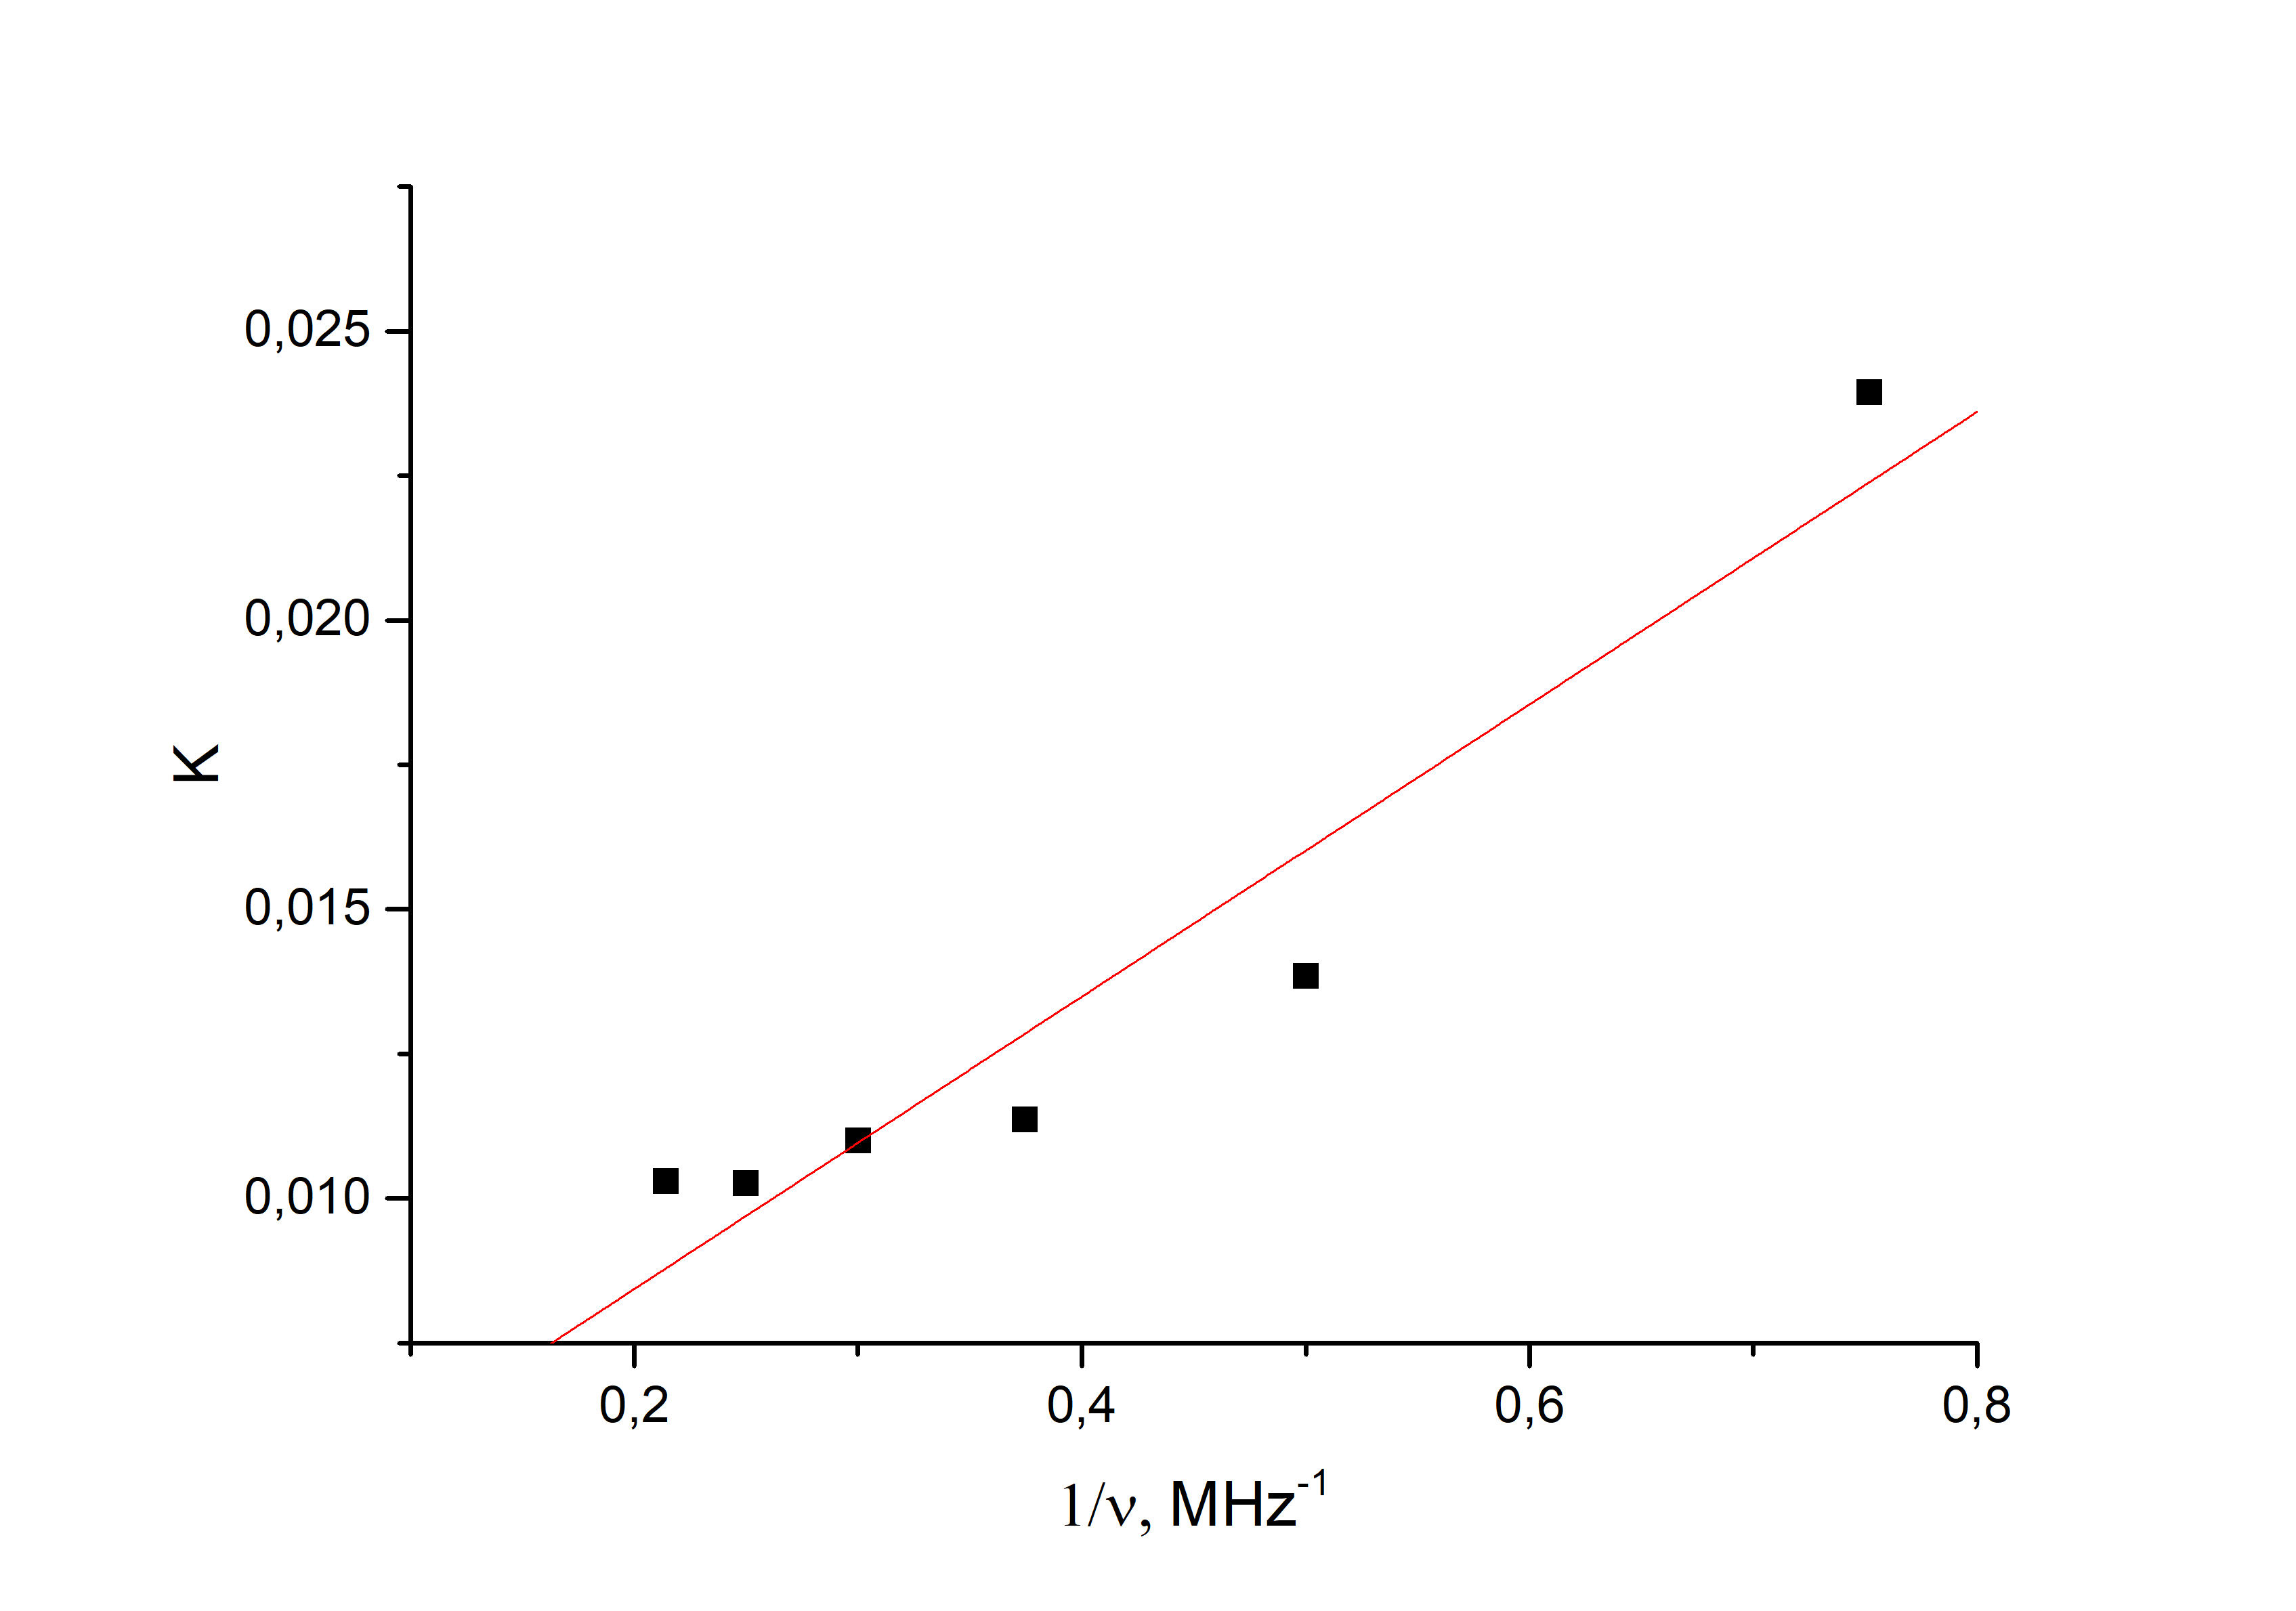
\includegraphics[width=0.45\linewidth]{p30}}
		\caption{График зависимости $K(\nu)$}
		\label{fig:p29}
	\end{figure}
		
		

\section{Выводы}

	В ходе работы были получены и исследованы спектры электрических сигналов различной формы. Кроме того
	
	\begin{itemize}
		\item проверено соотношение неопределённостей для последовательности прямоугольных импульсов и цугов,
		\item вычислена глубина амплитудной модуляции,
		\item проверено отношение амплитуд боковой и основной спектральной линии АМ-сигнала,
		\item показано, как потеря информации о фазе сигнала нарушает биективность преобразования Фурье на примере спектра фазово-модулированного сигнала, 
		\item сопоставлен спектр входа и выхода RC-цепочки,
		\item проверена зависимость амплитудного коэффициента фильтрации RC-цепочки от частоты,
		\item измерена постоянная времени RC-цепочки.	
	\end{itemize}
	 


\section{Приложение}

	\begin{figure}[h!]
		\centering
		\subfigure[$\nu_r = 2\ кГц, \tau = 50 \ мкс$]{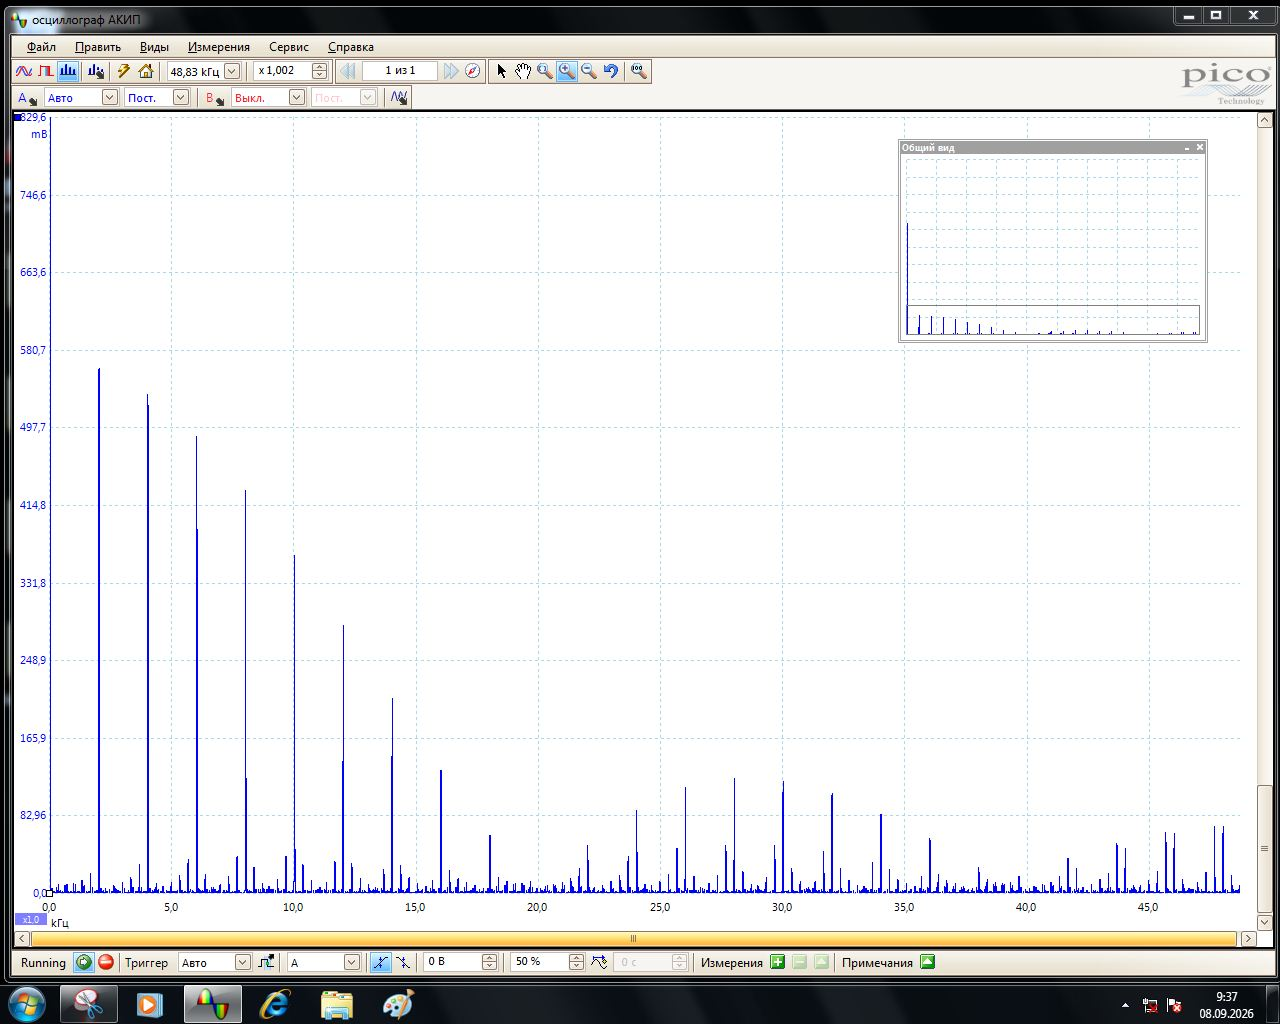
\includegraphics[width=0.45\linewidth]{2}}
		\subfigure[$\nu_r = 3\ кГц, \tau = 50 \ мкс$]{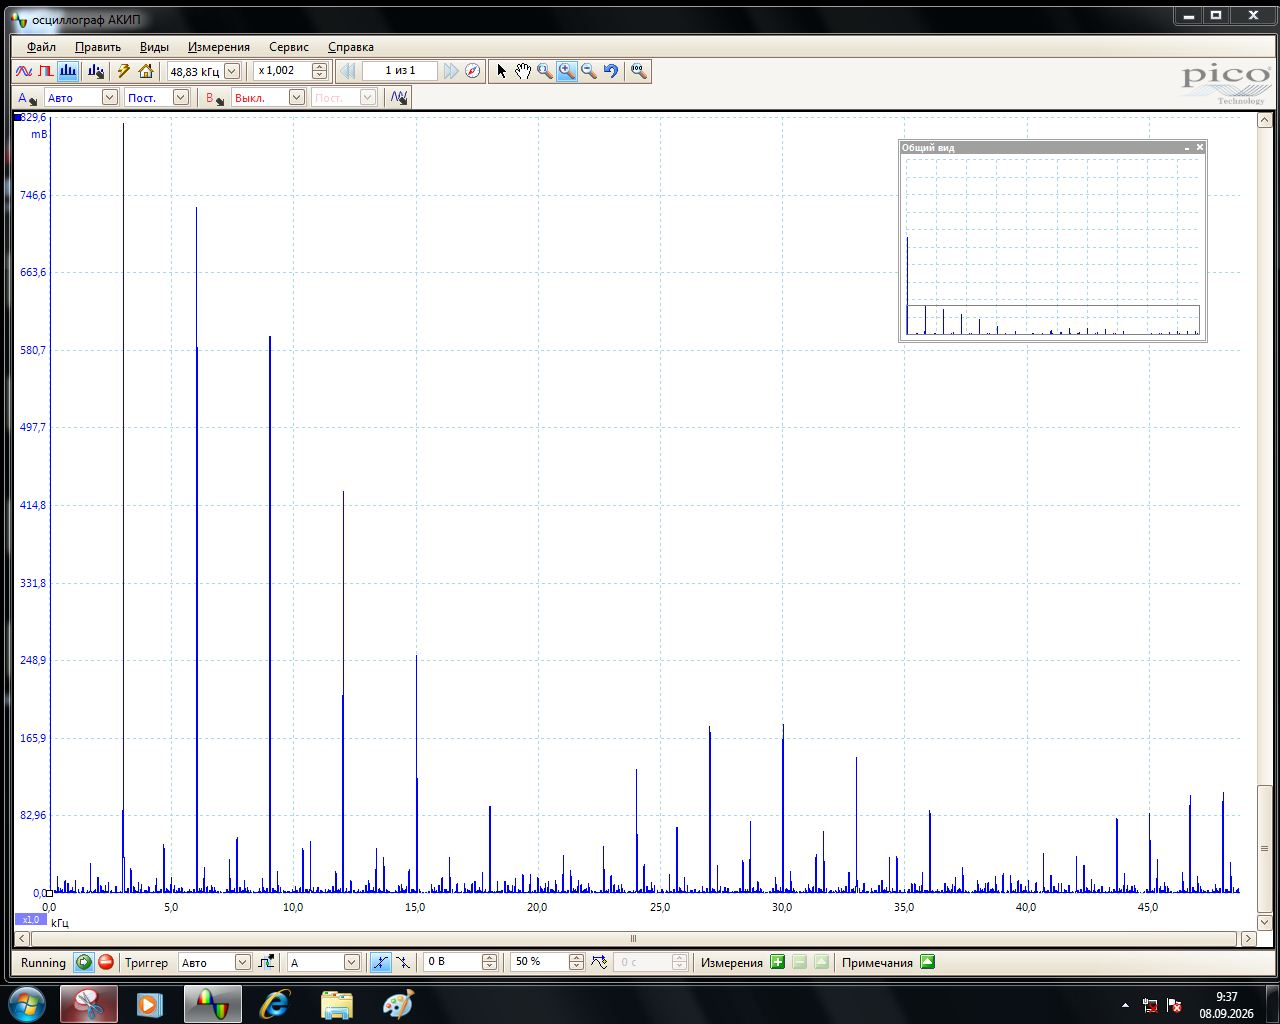
\includegraphics[width=0.45\linewidth]{3}}
		\subfigure[$\nu_r = 4\ кГц, \tau = 50 \ мкс$]{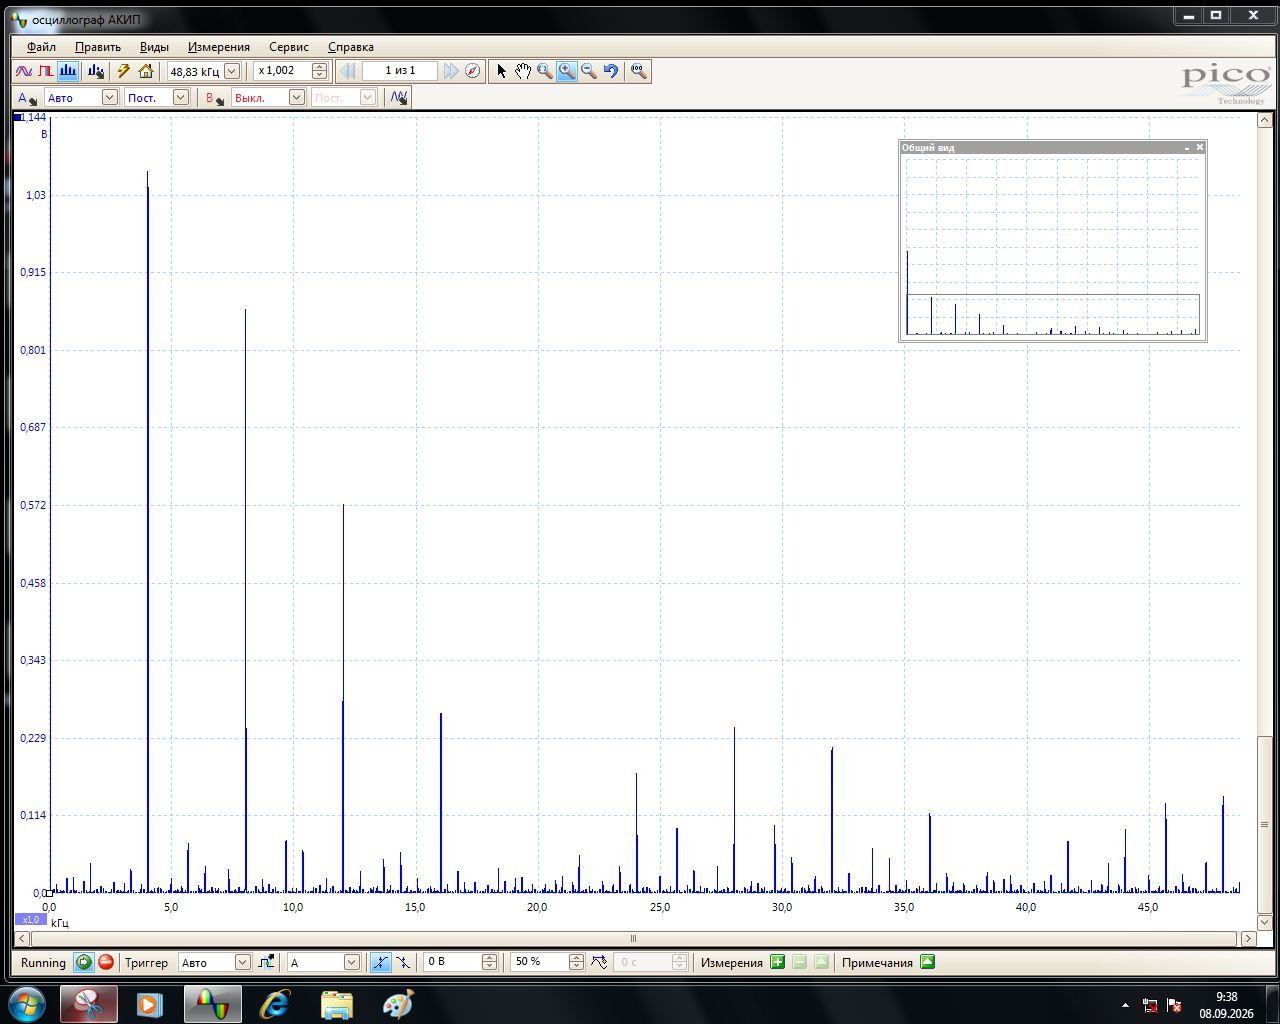
\includegraphics[width=0.45\linewidth]{4}}
		\subfigure[$\nu_r = 1\ кГц, \tau = 100\ мкс$]{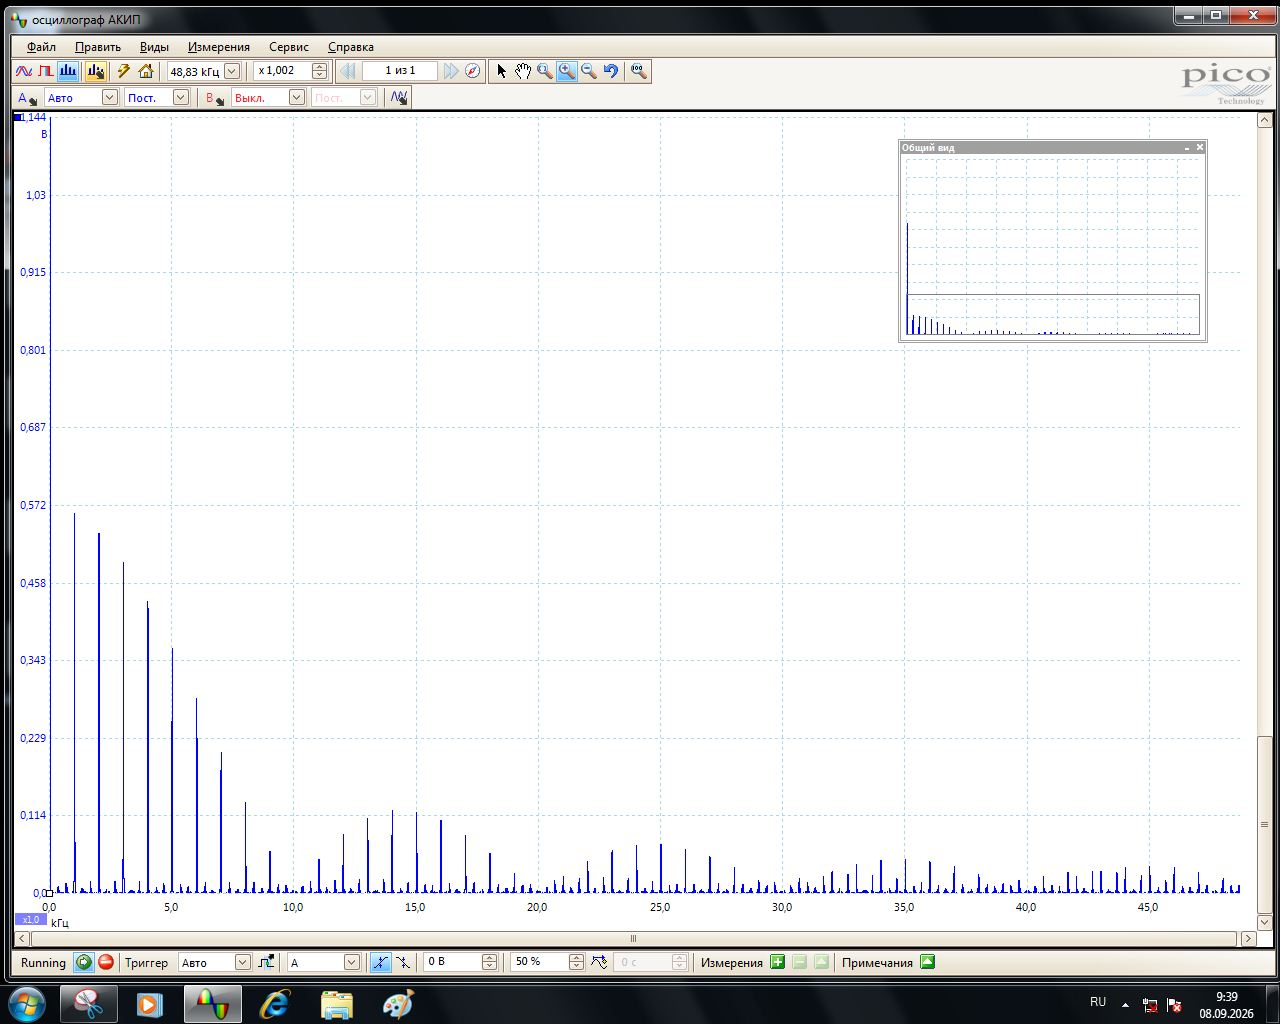
\includegraphics[width=0.45\linewidth]{5}}
		\subfigure[$\nu_r = 4\ кГц, \tau = 150\ мкс$]{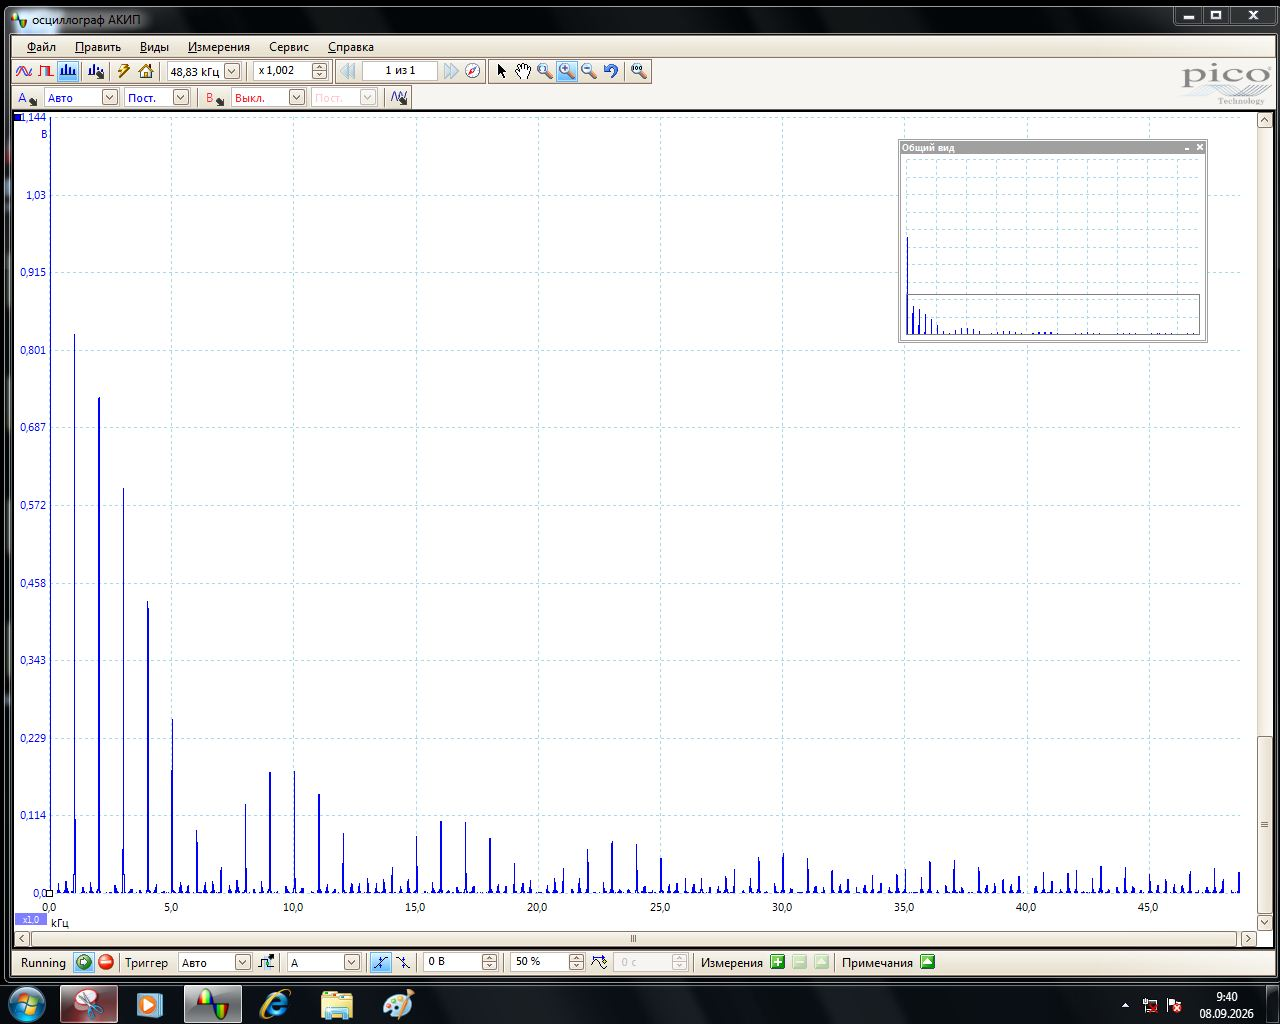
\includegraphics[width=0.45\linewidth]{6}}
		\caption{Спектры прямоугольных импульсов}
		\label{fig:p1}
	\end{figure}
	
	
	\begin{table}[h!]
		\centering
		\captionbox{Прямоугольные импульсы}{
		\begin{tabular}{|c|c|c|c|c|}
			\hline
			\rule[-1ex]{0pt}{2.5ex}  $\nu_r, \ кГц$	& $\tau, \ мкс$	&$\Delta \nu, \ кГц$	&$\delta \nu, \ кГц$  	& $\Delta \nu \cdot \tau$  \\
			\hline
			1  &50  &20  &1  	&1  \\
			\hline
			2  &50  &20  &2  	&1  \\
			\hline
			3  &50  &20  &3  	&1  \\
			\hline
			4  &50  &20  &4  	&1  \\
			\hline
			1  &100  &10  &1  	&1  \\
			\hline
			1  &150  &6,7  &1  	&1  \\
			\hline
			
		\end{tabular}}
	\end{table}
	
		\begin{table}[h!]
			\centering
			\captionbox{Амплитуды и частоты гармоник при $ T = 1 \ мс$, $ \tau = 50 \ мкс$}{
			\begin{tabular}{|c|c|c|c|c|c|c|}
				\hline
				n 	&1	&2	&3	&4	&5	&6  \\
				\hline
				$\nu_n^{эксп}, кГц$ 	&0,98	&2,01	&3,08	&3,99	&4,87	&5,01  \\
				\hline
				$\nu_n^{теор}, кГц$ 	&1,00	&2,00	&3,00	&4,00	&5,00	&6,00  \\
				\hline
				$|a_n^{эксп}|, усл. \ ед.$ 	&286	&281	&274	&268	&257	&246  \\
				\hline
				$|a_n^{теор}|, усл. \ ед.$ 	&498	&492	&482	&468	&450	&429  \\
				\hline
				$|a_n/a_1|^{эксп}$ 	&1,000	&0,982	&0,958	&0,937	&0,899	&0,860  \\
				\hline
				
				$|a_n/a_1|^{теор}$	&1,000	&0,988	&0,968	&0,940	&0,904	&0,861  \\
				\hline
				
				
		\end{tabular}}
	\end{table}
	
	\begin{table}[h!]
		\centering
		\captionbox{Изменение длительности импульса при $ T = 1 \ мс$}{
			\begin{tabular}{|c|c|c|c|c|c|c|c|}
				\hline
				$\tau, \ мкс$ 	&20	&25	&40	&50	&100	&150	&200  \\
				\hline
				$\Delta \nu, кГц$ 	&49,68	&39,71	&24,61	&19,98	&9,91	&6,84	&4,93 \\
				\hline	
		\end{tabular}}
	\end{table}
	
	\begin{table}[h!]
		\centering
		\captionbox{Изменение периода при $ \tau = 0,1 \ мс$}{
		\begin{tabular}{|c|c|c|c|c|c|c|}
				\hline
				$\nu$, кГц & 5 & 2 & 1 & 0,5 & 0,25 & 0,1 \\ 
				\hline
				$\delta \nu$, кГц & 5,028 & 1,935 & 1,011 & 0,509 & 0,250 & 0,198 \\ 
				\hline
		\end{tabular}}
	\end{table}
	
	
	\begin{figure}[h!]
		\centering
		\subfigure[$\nu_0 = 50\ кГц, T = 1 \ мс, \ N = 5$]{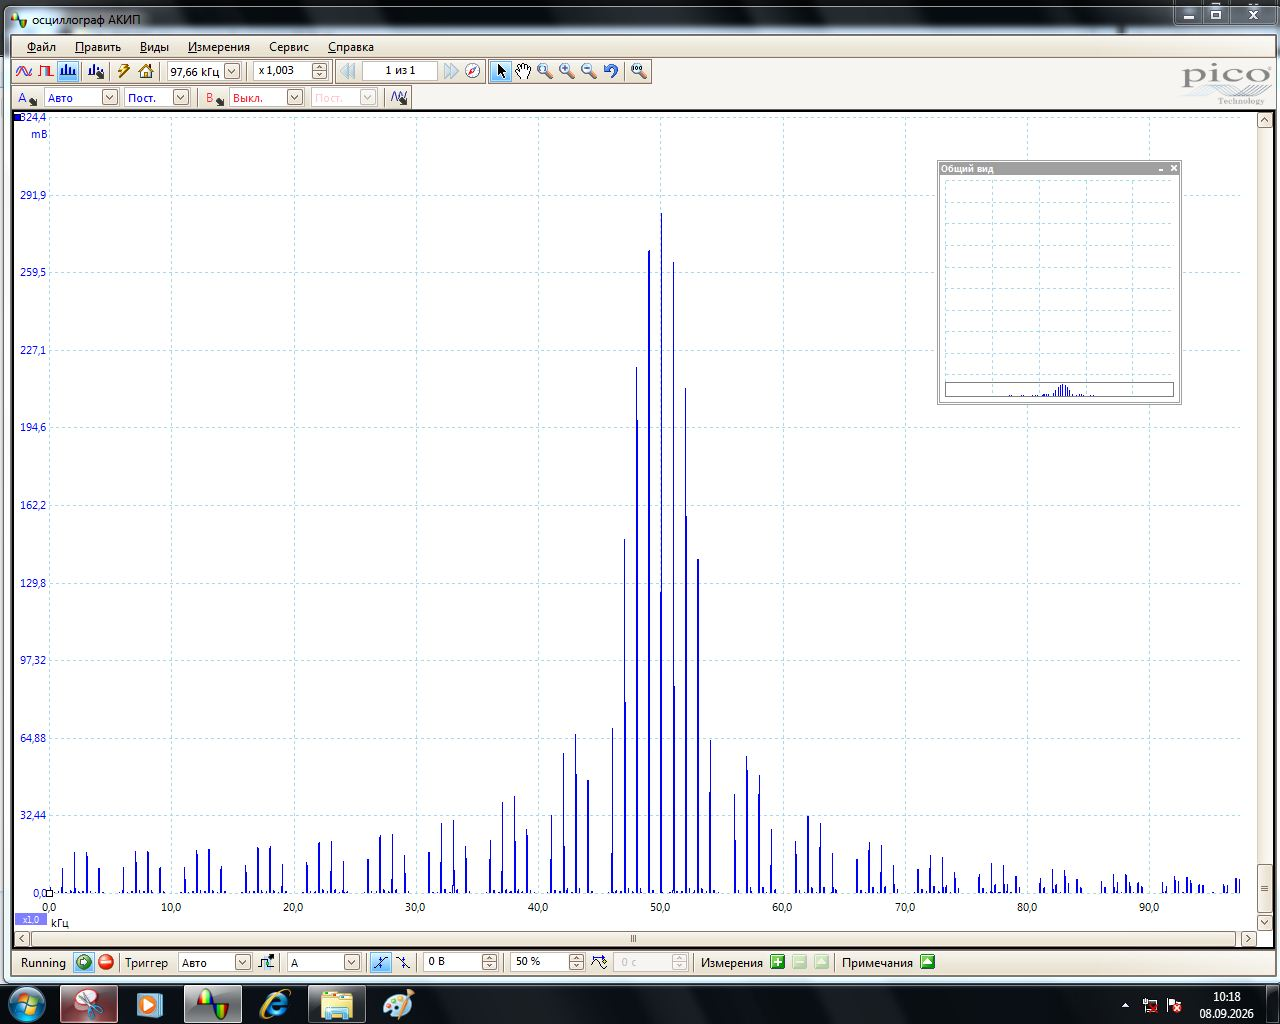
\includegraphics[width=0.45\linewidth]{16}}
		\subfigure[$\nu_0 = 50\ кГц, T = 1 \ мс, \ N = 10$]{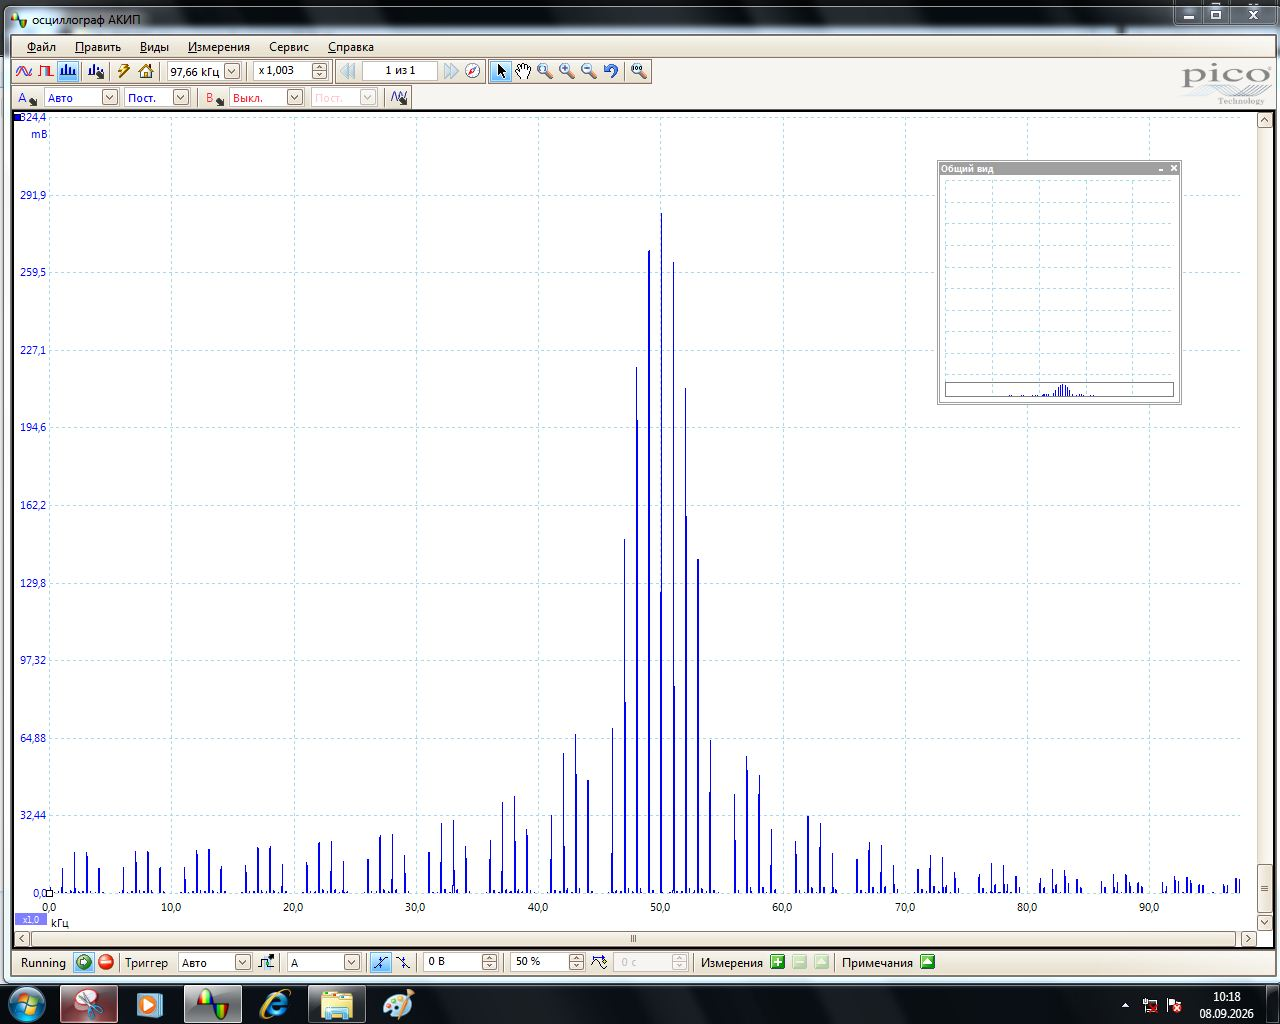
\includegraphics[width=0.45\linewidth]{16}}
		\subfigure[$\nu_0 = 30\ кГц, T = 1 \ мс, \ N = 5$]{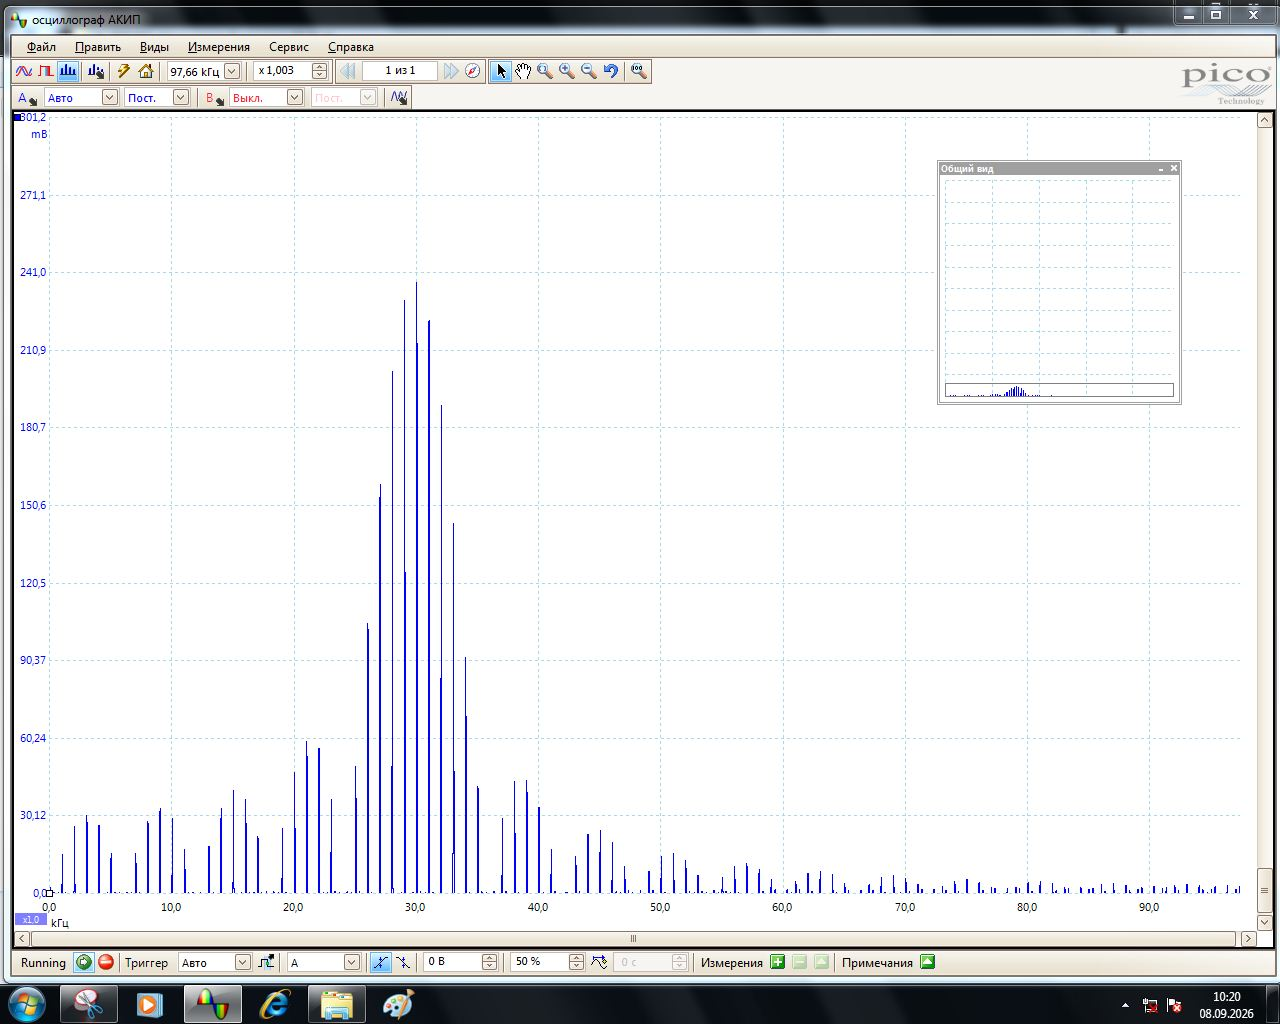
\includegraphics[width=0.45\linewidth]{19}}
		\subfigure[$\nu_0 = 50\ кГц, T = 2 \ мс, \ N = 5$]{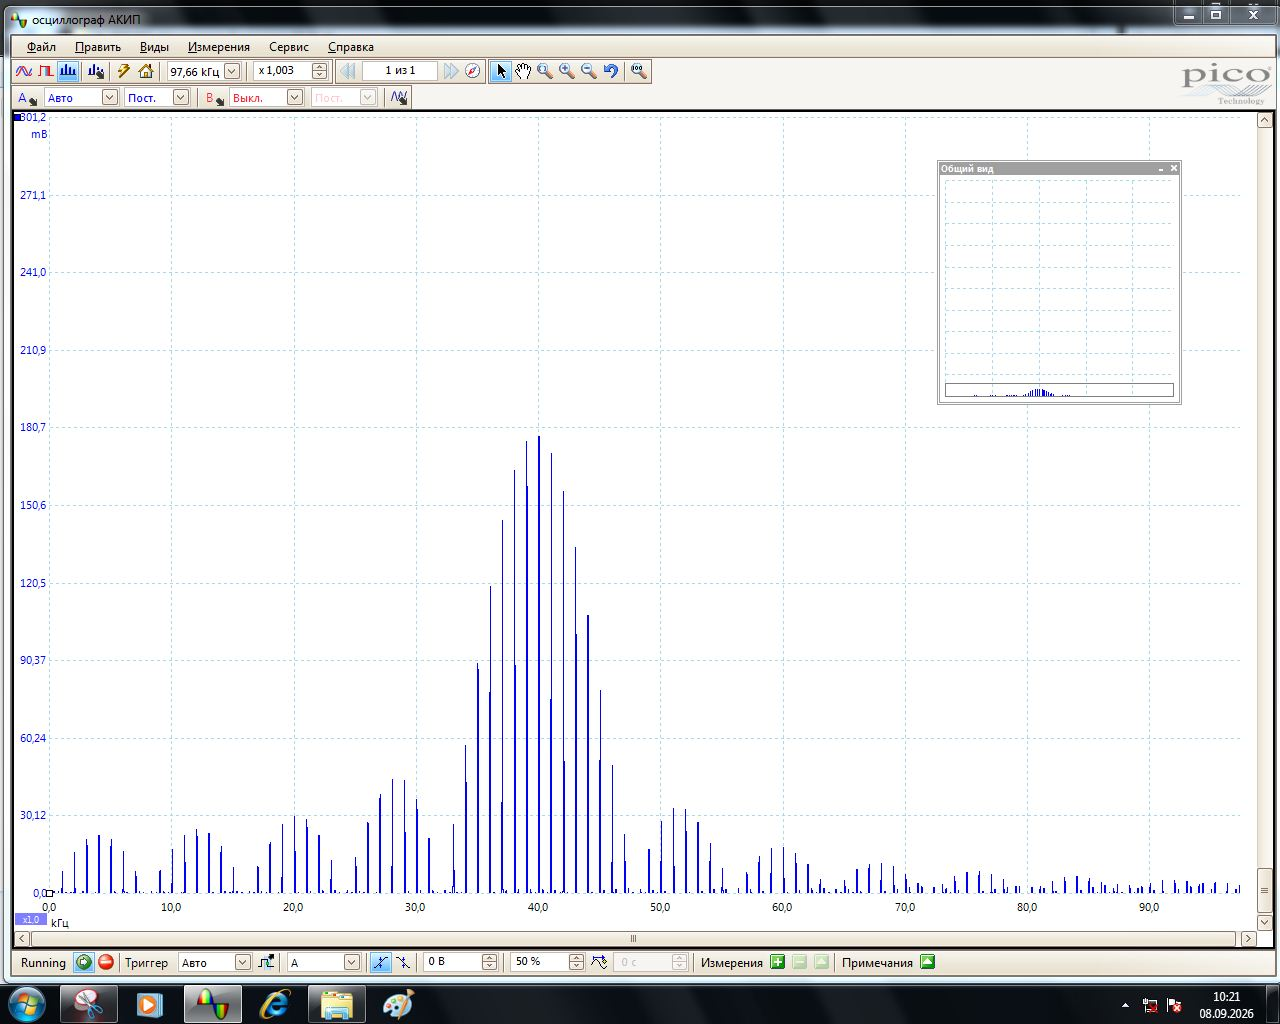
\includegraphics[width=0.45\linewidth]{20}}
		\caption{Спектры цугов}
		\label{fig:p2}
	\end{figure}
	
	
	\begin{table}[h!]
		\centering
		\captionbox{Коэффициент фильтрации RC-цепочки}{
			\begin{tabular}{|c|c|c|c|c|c|c|}
				\hline
				$\nu$, МГц & 1,33&	2,00&	2,67&	3,33&	4,00&	4,67
				 \\ 
				\hline
				$a_1$, усл.ед. &12,32&	6,34&	4,67&	3,97	&2,93&	2,17
				 \\ 
				\hline
				$a_2$, усл.ед. &514,6	&457,8	&411,1	&361,1	&285,7	&210,7
				
				\\ 
				\hline
				$K$ &0,0239&	0,0138&	0,0114&	0,0110&	0,0103&	0,0103
				
				\\ 
				\hline
		\end{tabular}}
	\end{table}




\end {document}